%%% Author: Steffen Walter  %%%
%%% Alias: firefly-serenity %%%
%%%%%%%%%%%%%%%%%%%%%%%%%%%%%%%%%%%%%%%%%%%%%%
%%%%%%%%%%%%%%%%%%%%%%%%%%%%%%%%%%%%%%%%%%%%%%
%%% DHBW Stuttgart compliant LaTeX tempalte
%%%%%%%%%%%%%%%%%%%%%%%%%%%%%%%%%%%%%%%%%%%%%%
%%%%%%%%%%%%%%%%%%%%%%%%%%%%%%%%%%%%%%%%%%%%%%

\documentclass[
book,
a4paper,   
titlepage,  
halfparskip,
12pt        
]{scrartcl}  

%%% packages selection for different purposes (see documentation of the package maintainer for more info)
\usepackage[ngerman]{babel,varioref}
\usepackage[utf8]{inputenc}
\usepackage[T1]{fontenc}
\setkomafont{sectioning}{\bfseries}
\usepackage{ae,aecompl}
%\usepackage{helvet}
%\renewcommand{\familydefault}{\sfdefault}
\usepackage{amsmath,amssymb,amstext}
\usepackage{psfrag}
\usepackage{listings}
\lstset{	
	language=bash,
	numbers=left,
	tabsize=2,
	stepnumber=1,
	breaklines=true,
	breakatwhitespace=false,
	backgroundcolor=\color{lightgray},		
} 
\newcommand\inline{\lstinline[basicstyle=\ttfamily]}
%\usepackage{units}
\usepackage[nottoc]{tocbibind}
\usepackage{cite}
\usepackage{caption}
\usepackage{tabto}
\usepackage{xcolor}
\usepackage{longtable}
\usepackage{lmodern}
\usepackage{setspace}
\usepackage{fancyhdr}
\usepackage{tablefootnote}
\usepackage{acronym}
\usepackage{varioref}
\usepackage[hyphens]{url}

%%%%%%%%%%%%%%%%%%%%%%%
%%%%%%%%%%%%%%%%%%%%%%%
%%% layout
%%%%%%%%%%%%%%%%%%%%%%%
%%%%%%%%%%%%%%%%%%%%%%%

% Enables blockset
\sloppy

\usepackage{geometry}
\geometry{a4paper, top=25mm, left=30mm, right=25mm, bottom=30mm, headsep=10mm, footskip=12mm}

%%% PDF options

\usepackage{ifpdf}

\ifpdf %if -> pdflatex
  \usepackage[pdftex]{graphicx}

  \pdfcompresslevel=9
  \usepackage[%
    pdftex=true,      
    backref,    
    pagebackref=false,
    colorlinks=false,
    hyperfootnotes=false,
    bookmarks=true,   
    bookmarksopen=false,
    bookmarksnumbered=false, 
    pdfpagemode=None,
    hidelinks
  ]{hyperref}
  \DeclareGraphicsExtensions{.pdf}
\else %else -> latex 
  \usepackage[dvips]{graphicx}
  \DeclareGraphicsExtensions{.eps}
  \usepackage[dvips, colorlinks=false]{hyperref}
\fi

%%% PDF-Meta-Information 
\hypersetup{
  pdftitle={T1000},
  pdfauthor={Steffen Walter},
  pdfsubject={Secrets Management in großen Firmenumgebungen},
  pdfcreator={Accomplished with LaTeX2e and pdfLaTeX with hyperref-package.},
  pdfproducer={science + computing ag},
  pdfkeywords={},
  breaklinks=true
}
\urlstyle{same}

% provides \AtBeginEnvironment, \patchcmd and \csdef:
\usepackage{etoolbox}

\makeatletter
\newcommand{\acroforeign}[1]{}

% patch the environment to print the foreign definition:
\AtBeginEnvironment{acronym}{%
	\def\acroforeign#1{ (#1)}%
}

% patch the acronym definition to safe the foreign definition:
\patchcmd\AC@@acro
{\begingroup}
{\begingroup\def\acroforeign##1{\csdef{ac@#1@foreign}{##1, }}}
{}
{}

% renew the first output to include the foreign definition if given:
\renewcommand*{\@acf}[1]{%
	\ifAC@footnote
	\acsfont{\csname ac@#1@foreign\endcsname\AC@acs{#1}}%
	\footnote{\AC@placelabel{#1}\hskip\z@\AC@acl{#1}{}}%
	\else
	\acffont{%
		\AC@placelabel{#1}\hskip\z@\AC@acl{#1}%
		\nolinebreak[3] %
		\acfsfont{(\acsfont{\csname ac@#1@foreign\endcsname\AC@acs{#1}})}%
	}%
	\fi
	\ifAC@starred\else\AC@logged{#1}\fi
}
\makeatother

%%%%%%%%%%%%%%%%%%%%%%%
%%%%%%%%%%%%%%%%%%%%%%%
%%% begin document
%%%%%%%%%%%%%%%%%%%%%%%
%%%%%%%%%%%%%%%%%%%%%%%

%%% header and footer before the actual body

\begin{document}

%%%%%%%%%%%%%%%%%%%%%%%
%%%%%%%%%%%%%%%%%%%%%%%
%%% titlepage
%%%%%%%%%%%%%%%%%%%%%%%
%%%%%%%%%%%%%%%%%%%%%%%

\begin{titlepage}
\begin{longtable}{lcr}
{
\includegraphics[height=1.7cm]{logo}} &
{
\includegraphics[height=1.05cm]{blank}} &
{
\includegraphics[height=1.7cm]{dhbw}}
\end{longtable}
% \enlargethispage{20mm}
\bigskip
\bigskip
\begin{center}
\vspace*{12mm} {\LARGE\bf Secrets Management in großen Firmenumgebungen}\\
\vspace*{12mm} {\large\bf Bericht Praxis I}\\
\vspace*{3mm} {\large\bf T1000}\\
\vspace*{12mm} des Studiengangs Informationstechnik (B.Sc.)\\ an der Dualen Hochschule Baden-Württemberg Stuttgart\\
% \vspace*{3mm} an der Dualen Hochschule Baden-Württemberg\\
\vspace*{12mm} von\\
\vspace*{3mm} {\large\bf Steffen Walter}\\
\vspace*{12mm} 03.09.2018\\
\end{center}
\vfill
\begin{spacing}{1.5}
\begin{tabbing}
mmmmmmmmmmmmmmmmmmmmmmmmmm \= \kill
\textbf{Bearbeitungszeitraum} \> 05.03.2018 - 04.05.2018\\
\textbf{Matrikelnummer, Kurs} \> 1145690, TINF17IN\\
\textbf{Ausbildungsunternehmen} \> science + computing ag, Tübingen\\
\textbf{Betreuer des Ausbildungsunternehmens} \>Dr. Marcus Camen\\
% \textbf{Gutachter der Hochschule} \> Bernd Beutlin\\
\end{tabbing}
\end{spacing}
\end{titlepage}

%%%%%%%%%%%%%%%%%%%%%%%
%%%%%%%%%%%%%%%%%%%%%%%
%%% Erklärung
%%%%%%%%%%%%%%%%%%%%%%%
%%%%%%%%%%%%%%%%%%%%%%%
%\thispagestyle{empty}
%
%\begin{table}[h]
%\centering
%  \begin{tabular}{| l |}
%  \hline
%  \\
%  \textbf{Erklärung} \\
%  \\
%  Ich versichere hiermit, dass ich meine Studienarbeit mit dem Thema: \\
%  ``Secrets Management in großen Firmenumgebungen`` selbstständig verfasst \\
%  und keine anderen als die angegebenen Quellen und Hilfsmittel benutzt habe. \\
%  \\
%  Ich versichere zudem, dass die eingereichte elektronische Fassung mit der gedruckten \\
%  Fassung übereinstimmt. \\ \\
%  ............................................................\hspace{0.5cm} %......................................\\
%  \textit{Ort} \hspace{1cm} \textit{Datum} \hspace{4.2cm} \textit{Unterschrift}\\
%  \\
%  \hline
%  \end{tabular}
%\end{table}
%\newpage

%%%%%%%%%%%%%%%%%%%%%%%
%%%%%%%%%%%%%%%%%%%%%%%
%%% Abstract
%%%%%%%%%%%%%%%%%%%%%%%
%%%%%%%%%%%%%%%%%%%%%%%
\thispagestyle{empty}

\large{\textbf{Zusammenfassung}}\\
\\
Das Thema Secrets Management wird zunehmend zu einem zentralen Thema in der
elektronischen Datenverarbeitung.  Unter dem Begriff ist im Folgenden vor
allem der Umgang mit geheimen Informationen gemeint.  Geheim sind
Informationen dann, sobald es schädlich ist wenn diese Informationen
Unbefugten zugänglich sind. Beispiele für derartige Informationen sind
Passwörter, geheime Schlüssel und geheime Dokumente. In der vorliegende Arbeit
wird herausgearbeitet welche Anforderungen große Unternehmen
an ihr Secrets Management stellen und welche Programme dabei häufig zum
Einsatz kommen. Weiterhin wird festgestellt welche
Anforderungen durch diese Programme \underline{nicht} erfüllt werden. Im Anschluss
wird eine voll umfängliche Secrets Management Software evaluiert und daraufhin beurteilt, 
ob Unzulänglichkeiten von gängiger Software behoben
werden können. 

Es wird außerdem betrachtet, welche neuen
Anforderungen Cloud Umgebungen mit sich bringen. Hierbei wird ein spezielles Augenmerk darauf gelegt,
welche Vorteile neuartige Software gegenüber herkömmlichen Lösungen bietet. 
In einer Gegenüberstellung mehrerer infragekommender Produkte wird dann erörtert warum Hashicorp Vault
eine sinnvolle Software zur Evaluierung darstellt. Für die Evaluierung wird dann eine virtuelle 
Umgebung erstellt, in der die Funktionen von Vault getestet werden.

Die Evalulierung führt zum Ergebnis, dass es sich bei Vault um eine brauchbare Sicherheitserweiterung handelt,
die sich beim Einsatz eines der unterstützen Authentifizierungssysteme leicht in bestehende Systeme integrieren lässt.
Es zeigt sich außerdem, dass die Schwächen herkömmlicher Softwarelösungen, vorwiegend in Bezug auf den Einsatz von Cloud-Diensten zum tragen kommen. Dementsprechend sind die Vorteile von Vault vor allem dann von Gewicht, wenn eine Verlagerung von Diensten in die Cloud stattfindet.
\newpage
\thispagestyle{empty}

\large{\textbf{Abstract}}\\
\\
The topic of secrets management is becoming an uprising matter in digital data processing.
In this report the term of secrets management is mainly used to describe the handling of confidential information.
Information is considered confidential, if it can be used to harm the owner of the secret in any way.  
Examples for information that meets this criteria would be password, private digital key or simply confidential documents.
This paper evaluates which requirements enterprises have for their secrets management and which software is currently used to try to fulfill those needs.
Subsequently the gaps between requirements and the functional range of the used software are being emphasized.
Furthermore a secrets management software with a modern approach is being examined to find out whether or not this software is able to fill in the gaps of traditional software.

Also the aspect of cloud environments is considered as a factor of importance. New challenges concering the work with cloud services are being worked out, to evaluate the differences between conventional and modern approaches. A comparison of such modern Software products reveals that Hashicorp Vault is the most sensible choice for an evaluation. To achieve the task of a practical evaluation of the software, a virtual environment is being set up.

The evaluation leads to the result, that Vault is a useful security extension. It can quite easily be integrated in existing environments, if one of the supported authentication systems is already in place. Another result of the evaluation is that there are several weaknesses of conventional software, that are mainly important when using cloud services. Accordingly the advantages of Vault are especially valuable when services are being shifted to the cloud.


%%%%%%%%%%%%%%%%%%%%%%%
%%%%%%%%%%%%%%%%%%%%%%%
%%% dictionaries
%%%%%%%%%%%%%%%%%%%%%%%
%%%%%%%%%%%%%%%%%%%%%%%

\pagestyle{fancy}
\fancyhf{} %% remove all previous settings

\newpage
\tableofcontents
\newpage
\pagestyle{fancy}
\fancyhf{} %% clear all previous settings
\fancyhead[R]{\thepage} %% pagenumber in the upper right corner
\fancyhead[L]{VERZEICHNISSE} %% section description in the upper left corner
\pagenumbering{roman}
\section*{Abkürzungsverzeichnis} %%Title for list of acronyms
\addcontentsline{toc}{section}{Abkürzungsverzeichnis}
\begin{acronym}[RADIUS]
 \acro{ACL}{Zugriffskontrollliste\acroforeign{engl. Access Control List}}
 \acro{AD}{Active Directory}
 \acro{API}{Schnittstelle zur Anwendungsprogrammierung\acroforeign{engl. Application Programming Interface}}
 \acro{AWS}{Amazon Web Dienste\acroforeign{engl. Amazon Web Services}}
 \acro{CA}{Zertifizierungstelle\acroforeign{engl. Certificate Authority}}
 \acro{CAE}{Rechnergestützes Entwicklung\acroforeign{engl. Computer Aided Engineering}}
 \acro{HCL}{Hashicorp Konfigurations Sprache\acroforeign{engl. Hashicorp Configuration Language}}
 \acro{IT}{Informationstechnik}
 \acro{JSON}{Java Script Objekt Notation}
 \acro{JWT}{\ac{JSON} Web Token}
 \acro{LCD}{Flüssigkristallanzeige\acroforeign{engl. Liquid Crystal Display}}
 \acro{LDAP}{Leichtgewichtiges Verzeichniszugriffsprotokoll\acroforeign{engl. Lightweight Directory Access Protocol}}
 \acro{MIT}{Massachusetts Institute of Technology}
 \acro{OECD}{Organisation für wirtschaftliche Zusammenarbeit und Entwicklung\acroforeign{engl. Organisation for Economic Co-operation and Development}}
 \acro{OIDC}{OpenID Connect}
 \acro{PKI}{Public Key Infrastruktur}
 \acro{RADIUS}{Authentifizierungsdienst für sich einwählende Benutzer\acroforeign{engl. Remote Authentication Dial-IN User Service}}
 \acro{SSL}{Spezifikation zur verschlüsselten Datenübertragung\acroforeign{engl. Secure Socket Layer}}
 \acro{TLS}{Transportschicht Sicherheit\acroforeign{engl. Transport Layer Security}}
 \acro{URL}{einheitlicher Ressourcenzeiger\acroforeign{engl. Uniform Resource Locator}}
 \acro{USA}{Vereinigte Staaten von Amerika \acroforeign{United States of America}}
\end{acronym}
\newpage
\setcounter{table}{0}
\listoffigures
\listoftables
\lstlistoflistings

%%%%%%%%%%%%%%%%%%%%%%%
%%%%%%%%%%%%%%%%%%%%%%%
%%% glossary
%%%%%%%%%%%%%%%%%%%%%%%
%%%%%%%%%%%%%%%%%%%%%%%
\newpage

\pagestyle{fancy}
\fancyhf{} %% clear all previous settings
\fancyhead[R]{\thepage} %% pagenumber in the upper right corner
\fancyhead[L]{GLOSSAR} %% section description in the upper left corner

\section*{Glossar} 
\addcontentsline{toc}{section}{Glossar}
\begin{acronym}
	\acro{Apache Webserver:}{ist nach dem Microsoft Webserver der zweithäufigsten Webserver im Internet\cite{apache} er läuft auf fast allen Platformen und gilt als robust und stabil. Außerdem hat der Apache Webserver einen sehr großen Funktionsumfang.\cite[S. 59]{apache2}}
	\acro{Authentifizierung:}{(v. griechischen „authentikos“ für Urheber, der Echte, der Wirkliche), bedeutet, eine Identität durch eine identitätsgebundene Information zu überprüfen und zu bestätigen.\cite[S. 127]{kerberos2}} 
	\acro{Authentisierung}{wird im englischen Sprachgebrauch mit Authentifizierung gleichgesetzt. In der deutschen Sprache meint Authentisierung die eigene Identität zu überprüfen.\cite[S. 127]{kerberos2}}
	\acro{Autorisierung:}{ist eine Berechtigung, eine ausdrückliche Zulassung, die sich normalerweise 1 auf einen Benutzer, bzw. auf eine Identität (Subjekt) bezieht. Autorisierung legt fest, was für wen in einem Netzwerk erlaubt ist und auf welche Ressourcen (Objekte) zugegriffen	werden darf.\cite[S. 159]{kerberos2}}
	\acro{CentOS Linux:}{ein Akronym für Community Enterprise Operating System. CentOS wird durch den Softwarehersteller Red Hat herausgebracht und ist eine lizenzkostenfreie Version von Red Hat Linux Enterprise.\cite[S. 1]{centos}}
	\acro{Chef:}{ist eine Automatisierungssoftware, die es sich zum Ziel gemacht hat, Infrastruktur als Code darzustellen. Die Konfiguration und Verteilung von Software in Cloudumgebungen, aber auch privaten Rechenzentren, kann durch Chef automatisiert werden.\cite{chef2}}
	\acro{Computercluster:}{eine Ansammlung von, meist identischer, Harware, welche zu einer logischen Einheit zusammengefasst wird. Der Cluster wird meist verwendet um komplexe Berechungen zu lösen, die auf einzenen Computern sehr lange dauern würde.}
	\acro{Crontab:}{kurz für chronograph table (etwa: Uhr Tabelle) ist ein Dienst zur Ablaufplanung einzelner Skripte. Mit gegebener Minute, Stunde, Tag, Woche, oder Monat wird eine regelmäßige Ausführung eins Skripts oder eines Kommanozeinbefehls ausgelöst.\cite[S. 212]{cron}}
	\acro{Dienst:}{eine autarke Einheit, welche eine spezifizierte Aufgabe bzw. Funktionalitaet erfuellt und diese ueber keine klar definierte Schnittstelle zur Verfuegung stellt}
	\acro{Docker:}{Docker ist eine technologie wie eingesetzt wird um eine Virtulisierung auf Betriebssystemebene zu erreichen. Diese Form der Virtualisierung ist bekannt unter der Bezeichnung Container. Es ist von zentraler Bedeutung diese Form der Virtualisierung von der Hardwarevirtulisierung abzugrenzen. Docker nutzt im gegensatz zur herkömmlichen Virtualisierung neben weiteren Betriebssystemkomponenten, vor allem den Linux Kernel um ihn zwischen mehreren virtuellen Containern zu teilen.\cite[S. 2]{docker2}}
	\acro{Hash:}{auch Hashwert genannt ist das Ergebnis einer Berechung aus einem Eingabewert und einer Hash-Funktion. Bei gängigen Hashfunktionen kann mit einer sehr hohen Wahrscheinlichkeit davon ausgegangen werden, dass jede unterschiedliche Eingabe einen anderen Hashwert als Ergebnis hat. Die gleiche Eingabe liefert jedoch immer den gleichen Hash. Aus dem Hashwert ist es, je nach Komplexität der Hashfunktion, nur mit sehr großem Aufwand möglich auf den Eingabewert zu schließen.\cite[S. 93ff]{hash}}
	\acro{KeePass Passwort Safe:}{ein quelloffener Passwortmanager, dazu designed wurde viele Passörter auf sichere Art und Weise zu speichern. Der Zugang zu diesem Passwortsafe wird allein durch ein einziges Masterpasswort gewährt.}
	\acro{Kubernetes:}{ist eine quelloffene Software, die dazu verwendet wird Dockercontainer zu verwalten. Dabei führt Kubernetes eine weitere Abstraktionsebene ein und kapselt jeden Dockercontainer noch einemal in einen sogenannten Pod. Pods machen es Kubernetes sehr einfach Dockercontainer auf Computerclustern auszuführen, wobei es keine Rolle spielt auf welchem Server der Container letztendlich ausgeführt wird.\cite{kubernetes}}
	\acro{Microservice:}{ein Software Baustein, der genau eine Aufgabe erledigt. Er kann bei bedarf gestartet und skaliert werden. Idealerweise sind sie Fehlertolerant und bieten Möglichkeiten bei fehlern auf eine weitere Instanz des gleichen Services zurückzugreifen.\cite[S. 6]{micro}}
	\acro{OpenStack:}{der Markenname eines quelloffenen Betriebssystems welches entwickelt wurde um eine Cloud Computing Infrastruktur bereit zu stellen.\cite[S. 2]{barbican}}
	\acro{Skalierbarkeit:}{die Fähigkeit eines Systems zur flexiblen Änderung ihrer Größe. Der Begriff wird meist dann verwendet wenn es um ein Ausweitung des gefragten Systems geht.}
\end{acronym}

\newpage
\begin{onehalfspacing} %% set space between lines to 1.5
\pagestyle{fancy}
\fancyhf{} %% remove all previous settings
%\renewcommand{\headrulewidth}{0pt} %%% activate to remove seperation line between head and main body
\fancyhead[L]{\rightmark} %% section name and number in the upper left corner
\fancyhead[R]{\thepage} %% pagenumber in upper right corner
\pagenumbering{arabic}

%%%%%%%%%%%%%%%%%%%%%%%
%%%%%%%%%%%%%%%%%%%%%%%
%%% begin main document
%%%%%%%%%%%%%%%%%%%%%%%
%%%%%%%%%%%%%%%%%%%%%%%

\section{Einleitung}
\label{subsec:einfuehrung}
Mit der fortschreitenden Digitalisierung nahezu aller Wirtschaftszweige steigt auch die Relevanz für die Absicherung der daraus resultierenden \ac{IT}-Infrastrukturen. Zusätzlich zu den eigenen Sicherheitsbelangen des Betreibers einer informationstechnischen Umgebung kommen noch gesetzliche Regelungen wie zum Beispiel das Gesetz zur Erhöhung der Sicherheit informationstechnischer Systeme (IT-Sicherheitsgesetz)\cite{gesetz} zum Tragen. 
Vor allem im Bezug auf eine zunehmende Verlagerung des \ac{IT}-Betriebs hin zum Cloud Computing und den damit verbundenen Problemen dezentraler Datenhaltung (im speziellen bei den public und hybrid Modellen, siehe Kapitel \vref{subsec:cloud}), entstehen häufig unübersichtliche Sicherheitskonzepte. Durch die große Varianz der Szenarien, bei unterschiedlichen Sicherheitsniveaus der Daten, sind die verwendeten Konzepte sehr unterschiedlich.\cite[S. 7f]{risiko}\\
Spionage- und Sabotage-Angriffe werden aus den unterschiedlichsten Motivationen und auch von den unterschiedlichsten Subjekten verübt. So reicht das Spektrum der Angreifer von Kleinkriminellen über Geheimdienste und Terroristen bis hin zur organisierten Kriminalität. Die Aufgabe der \ac{IT}-Sicherheit besteht darin, die potentiellen Angreifer in ihren Erwägungen zu berücksichtigen und die Werte und Geheimnisse der Unternehmen zu schützen. Ein zentraler Faktor bei der Entwicklung eines Sicherheitskonzepts auf dieser Grundlage ist es, ein stringentes Konzept zur Kontrolle der Autorisierung einer Person oder eines Dienstes beim Zugriff auf die verschiedenen Bereiche in der betreuten Umgebung auszuarbeiten. Neben der Autorisierung spielt auch die Authentifizierung eine wichtige Rolle, denn es muss zu jedem Zeitpunkt sichergestellt werden, dass die Autorisierung auch der richtigen Person oder Anwendung übertragen wird.\cite[S. 9]{risiko}\\
Der Aufwand, welcher für \ac{IT}-Sicherheitskonzepte betrieben wird bemisst sich meistens am Schaden, der zu erwarten ist, sollten geheime Daten in die Hände Dritter gelangen. Die Kosten die durch Angriffe auf Computersysteme entstehen, lassen sich von einer wissenschaftlichen Perspektive nur schwer quantifizieren, denn Unternehmen veröffentlichen nur sehr selten Daten zu den Schäden, die durch Angriffe verursacht wurden. Die Gründe dafür sind mutmaßlich Angst vor Imageschäden oder schlicht das Fehlen von Daten, weil keine Überwachung stattfindend. Da durch diesen Missstand die Quantifizierung eines möglichen Schadens oft nicht möglich ist, werden häufig erst gar keine Sicherheitsmaßnamen ergriffen \cite{spionage}. Generell gibt es verschiedene Faktoren die bei der qualitativen Kostenabschätzung berücksichtigt werden müssen, so wird im Allgemeinen zwischen direkten und indirekten Kosten unterschieden.\cite[S. 12]{kosten}
\subsection{Direkte Kosten}
Die direkten Kosten die durch Wirtschaftsspionage entstehen können, bemessen sich zu allererst an dem direkten Wert des gestohlenen Eigentums. Dieser Wert lässt sich durch den finanziellen Gegenwert, den das Eigentum hat ermitteln und an den zu erwartenden Gewinneinbußen durch den Verlust (der Exklusivität) des Eigentums. Weiterhin entstehen direkte Kosten durch das Desaster-Recovery, das heißt durch die Schritte die eingeleitet werden müssen um den Status Quo von vor dem Angriff wieder herzustellen. Zu guter Letzt werden noch diejenigen Kosten hinzugezählt, die durch die Prävention einer Wiederholung des Ereignisses entstehen, dazu zählen Prozessänderungen, Sicherheitsunterweisungen und ähnliche direkte Maßnahmen.\cite[S. 13]{kosten}
\subsection{Indirekte Kosten}
Zu den indirekten Kosten werden die Umsatzausfälle durch Image- und Markenschäden gezählt. Außerdem können hohe Umsatzeinbußen durch Plagiate entstehen, welche in Folge des gestohlenen Eigentums verbreitet werden. Plagiate können deutlich günstiger angeboten werden, da die Kosten für Forschung und Entwicklung nicht in den Preis eingerechnet werden müssen.\cite[S. 14]{kosten}
\subsection{Versuch einer Quantifizierung}
Nach Schätzungen der \ac{OECD} belaufen sich die Schäden durch Fälschungen und Produktpiraterie weltweit auf 638 Milliarden US-Dollar pro Jahr. Die Schätzungen diesbezüglich gehen aber weit auseinander. Es scheint jedoch sicher zu sein, dass sich die Schäden im dreistelligen Milliardenbereich bewegen. Für die deutsche Wirtschaft liegen die Schätzungen zwischen 20 und 50 Milliarden Euro jährlich.\cite[S. 16f]{kosten}
\subsection{Anforderung an Sicherheitssoftware}
\label{subsubsec:anforderung}
Die Inhalte diese Kapitels werden in Anlehnung an interne Dokument eines großen Unternehmens und Gesprächen mit \ac{IT}-Administratoren herausgearbeitet.

Spezifische Anforderungen die an eine Software zum Secrets Management gestellt werden, können wie folgt zusammengefasst werden:

\begin{itemize}
  \item Auffindbarkeit - Es muss zu jedem Zeitpunkt möglich sein, ein gewünschtes Objekt zu lokalisieren.\cite[S. 3]{kerberos2}
  \item Nachvollziehbarkeit - Um regelmäßige Audits durchzuführen (wie zum Beispiel durch die Zertifizierung nach ISO 27001 vorgesehen\cite[S. 17]{risiko}) muss es möglich sein durch Protokolldaten die Nachvollziehbarkeit der Abläufe zu gewährleisten.
  \item Break Glass Szenario - Die Möglichkeit einen Benutzeraccount, oder ein ganzes System zu sperren muss gegeben sein. Zu diesem Zweck muss es unter Umständen möglich sein normale Zugriffskontrollabläufe zu umgehen um eine schnelle Reaktion gewährleisten zu können.\cite{break}
  \item Hochverfügbarkeit - Eine maximal hohe Verfügbarkeit soll durch geeignete Mechanismen bereitgestellt werden.\cite[S. 3]{ha} 
  \item Integrität - Daten müssen vollständig, konsistent und akkurat sein. Daraus ergeben sich dem US-amerikanischen Gesundheitsministerium zufolge, diese Bedingungen: Daten müssen zuschreibbar, lesbar, parallel aufgezeichnet, original oder eine echte Kopie sein.\cite[S. 2]{health}
  \item Verlässlichkeit - Daten müssen authentisch sein. Das heißt es muss verhindert werden, dass sie durch Unbefugte verändert werden.
  \item Autorisierung - Der Zugriff auf Daten soll nur dann möglich sein, wenn die betroffene Person/Maschine berechtigt ist (minimale Berechtigungsvergabe). Zugriffskonzepte werden nach dem Prinzip Need-to-know gestaltet, das bedeutet Zugriffserlaubnisse werden nur dann erteilt wenn die Identität die Berechtigung tatsächlich braucht.
  \item Benutzerfreundlichkeit - Unkomplizierter Zugriff auf die Computersysteme durch jede Identität.
  \item Authentifizierung - Sichere Anmeldeverfahren, zur Validierung der Identität,  müssen zur Verfügung stehen.
\end{itemize}

Rechtliche Aspekte werden durch den Vorliegenden Bericht nicht weiter beleuchtet, da der Fokus dieser Arbeit auf der technischen Umsetzung liegt. Verwertbare juristische Einschätzungen müssen in Zusammenarbeit mit Rechtsgelehrten erstellt werden.
\newpage

\section{Grundlegende Informationen}
\label{sec:inf}
Dieses Kapitel beschreibt die Motivation und die Umgebung in die das Projekt eingebettet ist. Das Kapitel soll außerdem ein Grundverständnis der Arbeitsumgebung und der verfolgten Agenda vermitteln.

\subsection{Motivation}
In Kapitel \vref{sec:grund} werden Problematiken und Widersprüche aufgezeigt, die zur Wahl des Themas für die vorliegende Arbeit geführt haben. Der Diskurs um Sicherheits- und Secrets- Management in großen Firmenumgebungen und der Trend hin zur Auslagerung eigener Rechenzentren zu Cloud-Providern, wirft die Frage nach funktionierenden Sicherheitskonzepten auf. Nicht zu Letzt, die zunehmenden erfolgreichen Angriffe, die auf ein unzureichendes Sicherheitskonzept zurückzuführen sind werfen die Frage nach einem umfangreichen Sicherheitssystem auf, welches dazu in der Lage ist neue Bedrohungen und sich verändernde Bedingungen abzudecken.\\
Eine der wichtigsten Herausforderungen bei Cloudumgebungen stellt nicht allein das Management der Zugangsdaten von Benutzern dar, es wird immer wichtiger auch die Verwaltung von Diensten und deren Zugangsdaten zu beleuchten. Ein beliebter Einstiegspunkt für Angreifer, sind Passwörter, die im Klartext oder mit minderwertiger Verschlüsselung in Skripten, Konfigurationsdateien oder im Programmcode eingebettet sind. Häufig sind derartige Konfigurationen dort zu finden, wo Dienste zum Beispiel auf Datenbanken zugreifen müssen. Im Cloudumfeld wo eine Vielzahl von Microservices die Regel ist, verschärft sich dieses Problem noch einmal.\\
Auf Grund der Problematiken die in Kapitel \vref{subsec:pass} aufgezeigt werden und denen die in diesem Kapitel beschrieben sind, kann ein dringender Handlungsbedarf ausgemacht werden. Dabei muss ist es das Ziel die Vereinbarkeit von administrativem Aufwand und ausreichender Absicherung von zentraler Bedeutung

\subsection{Projektumgebung}
\label{subsec:proj}
Das Thema Sicherheit in der Datenverarbeitung ist ein zentrales Thema in der \ac{IT}. Über die Jahre haben sich die Möglichkeiten zur Absicherung informationstechnischer Systeme stetig weiterentwickelt, sodass die Absicherung von Computern, Netzwerken, Servern und ganz allgemein Informationen zu einem wichtigen Zweig der Branche geworden ist. Mit jeder Einführung von neuen Technologien stellt sich immer auch die Frage nach den Sicherheitsfunktionen.\\
Cloud Computing ist aktuell eine sehr wichtige und schnell wachsende Technologie in der \ac{IT}-Branche. In den \ac{USA} werden Technologien rund um das Thema Cloud stark gefördert und es gibt eine Vielzahl an Softwareprodukten die sich diesem Feld verpflichtet haben. Für die Nutzung der Vorteile dieser Technologien gibt es einige Faktoren die es zu betrachten gilt. Zum Beispiel gilt es zu kalkulieren, ob eine Verlagerung von Anwendungen oder Daten auf Cloud Infrastruktur wirtschaftlich ist oder nicht. Dabei spielt die vorhandene Infrastruktur eine Zentrale Rolle und es muss abgewägt werden ob ein schrittweiser oder teilweiser Umzug der zu betreibenden Dienste, in Betracht kommt. Vor diesem Hintergrund spielt das Thema Sicherheit eine wichtige Rolle. Daten auf ``fremder`` Hardware zu speichern, wie es in Cloud Umgebungen gängige Praxis ist, stellt ein Risiko dar. Es muss darauf geachtet werden, dass kritische Daten und Anwendungen nur autorisierten Identitäten (siehe \vref{subsec:ident}) zugänglich sind. Weiterhin ist abzuwägen in wie fern sich die aktuelle Software, welche zur Authentifizierung und Autorisierung eingesetzt wird, dazu eignet die genannten Herausforderungen zu bewältigen. In dieser Arbeit sollen Aspekte wie dieser genauer beleuchtet werden.

\subsubsection{Unternehmensvorstellung}
Die science + computing ag, kurz s+c, ist als Tochtergesellschaft der ATOS SE ein Unternehmen des \ac{IT}-Dienstleistungs- und Consultingbereichs. Mit seinen knapp 400 Mitarbeitern betätigt sich die s+c hauptsächlich in den Bereichen High Performance Computing, \ac{IT}-Sicherheit, 3D-Virtualisierung und System-Management. Durch OpenSoftware-Dienstleistungen und diverse Softwareprodukte betätigt sich das Unternehmen zudem im Bereich der Softwareentwicklung. Neben Großkunden der Automobilindustrie besteht der diverse Kundenkreis der s+c aus Mikroelektronikherstellern, Chemie- und Pharmaunternehmen, Maschinen- und Anlagenbauern, Forschungs- und Bildungseinrichtungen sowie Unternehmen aus der Luft- und Raumfahrtbrache.\\
Zum Hauptsitz in Tübingen kommen noch vier weitere Standorte in Berlin, Düsseldorf, Ingolstadt und München hinzu. Bis zur Übernahme durch den französischen Computerhersteller Bull war die 1989 gegründete science + computing ag ein eigenständiges Unternehmen.\cite{bull} Im Jahr 2014 wurde die BULL-Gruppe ihrerseits durch die ATOS SE übernommen wodurch auch die science + computing ag nun zum ATOS-Gesamtkonzern gehört.\cite{atos}\\
ATOS SE ist ein International agierender Konzern mit knapp 100.000 Mitarbeitern, einem jährlichen Umsatz von 14 Milliarden Dollar und Hauptsitz in Bezons (Frankreich). Nach der Forbes Liste der 2000 größten Unternehmen der Welt belegt ATOS SE mit den oben genannten Werten den Platz 858 (Stand Juni 2018).\cite{forbes} Im Zuge der Übernahme durch ATOS SE wird die Marke s+c seit 2016 nicht mehr weitergeführt. Stattdessen wird nun die Konzernmarke ATOS verwendet.

\subsubsection{Arbeitsumgebung}
Die Durchführung der Projektarbeit findet in einem der Teams des Bereiches \ac{CAE} der science + computing ag statt. Im Team \ac{CAE}3 werden Kunden betreut, die unter Verwendung von High Perfomance Computing Berechnungen durchführen. Der Fokus des Teams liegt dabei auf Kundenkreisen die sich im Bereich \ac{CAE} betätigen. Im Team gibt es verschiedene Kompetenzen um die volle Bandbreite der Kundenwünsche abdecken zu können. Zu den Kernkompetenzen gehören hierbei die Entwicklung von systemunterstützender Software, Administration von Computerclustern inklusive Überwachung der Systemkomponenten sowie Administration und Bereitstellung von speziellen Speicherinfrastrukturen.\\
Die Evaluierung welche Teil dieses Praxisberichts ist, soll erste Informationen liefern aus denen sich die Nutzbarkeit von Secrets Management Software zur interne Nutzung ableiten lässt. Der praktische Teil der Evaluierung wird auf einer virtualisierten Umgebung auf Basis von VMware Workstation durchgeführt.

\subsubsection{Unternehmensspezifische Anforderungen}
Bei s+c gibt es laufend Projekte, die sich mit zukunftsweisenden Technologien beschäftigen, um eine Übernahme in das Leistungsportfolio der Firma zu erörtern. Bei den Projekten geht es sowohl um die Verbesserung eigener Geschäftsprozesse und Arbeitsabläufe als auch um die Optimierung der Leistungen gegenüber dem Kunden. Wichtige Faktoren die bei einer derartigen Einschätzung betrachtet werden müssen sind Einsatzmöglichkeiten, Einsatzbereiche, Kosten, Schnittstellen und Skalierbarkeit. 
                                                                                                          
Dem Trend zu einheitlichen Arbeitsmitteln folgend ist der Einsatzbereich so weit wie möglich zu wählen, ohne dabei jedoch die einzelnen Bereiche in ihrer Arbeit zu beeinträchtigen. Für das vorliegende Projekt gilt, dass nach erfolgreicher Evaluierung ein produktives Pilotprojekt in einem definierten Umfeld gestartet werden kann. Zum Zweck der Evaluierung soll eine Testversion oder die kostenfreie Version des Secrets Management Systems Hashicorp Vault eingesetzt werden dessen Auswahl in Kapitel \vref{sec:eval} begründet wird.\\
Um qualifizierte Aussagen über den Aufwand treffen zu können ist es wichtig die Schnittstellen zu bestehenden Systemen zu bewerten und auf ihre Funktionalität hin zu untersuchen. Das Secrets Management Konzept ist derart anzulegen, dass es sich möglichst einfach in eine bestehende Umgebung integrieren lässt. Bei der Evaluierung muss auch darauf geachtet werden ob sich die Secrets Management Software zum Einsatz in Großunternehmen einsetzten lässt. Es ist von Vorteil wenn die Software die Funktion mitbringt, über mehrere Hardwareinstanzen hinaus erweiterbar zu sein. Außerdem ist zu betrachten ob das System auch rechenzentrenübergreifend eingesetzt werden kann.

\newpage
\section{Theoretische Grundlagen}
\label{sec:grund}
Das folgende Kapitel liefert die theoretischen Grundlagen für die praktische Umsetzung der Projektarbeit. Es wird eine breite Übersicht über den Themenkomplex des Secrets Management gegeben und es wird gezeigt welche Softwareprodukte aktuell in Unternehmen zum Einsatz kommen um Probleme die mit den Themenkomplexen Authentifizierung und Autorisierung in Verbindung stehen zu lösen. Außerdem wird aufgezeigt welche neuen Herausforderungen das Arbeiten unter Verwendung von Cloud Computing mit sich bringt. 

\subsection{Das Passwort}
\label{subsec:pass}
Das Passwort ist die einfachste und am häufigsten verwendete Methode um eine Authentifizierung zwischen einem Mensch und einem Computersystem durchzuführen. Es ist leicht zu implementieren und zu bedienen. Es gibt allerdings eine Reihe von Angriffsszenarien bei denen das klassische Passwort als authentifizierender Faktor versagt.
\begin{itemize}
	\item Passwörter können über sogenannte Brute-force Angriffe ``erraten`` werden. Um diese Angriffe durchzuführen gibt es spezielle Programme, die so lange alle möglichen Kombinationen von Tastatureingaben ausprobieren, bis sie das Passwort herausgefunden haben. Passwörter und Passworthashes werden häufig im Klartext in Datenbanken abgelegt, was regelmäßig dazu führt, dass Datenbanken gehackt werden. Die darin gespeicherten Passwörter werden dann durch die Brute-force Methode aus den Hashes ermittelt. Mit aktueller Hardware ist der Rechenaufwand verhältnismäßig gering.\cite{brute}  
	\item Das Passwort kann beim Eintippen durch einen Dritten gesehen oder gefilmt werden. 
	\item Wenn Passwörter über ein Netzwerk übertragen werden, können sie durch spezielle Software abgegriffen werden. Außerdem gibt es Software, welche die Tastatureingaben am Computer protokollieren kann. Solche Programme können dazu verwendet werden Passwörter die an betreffenden Endgeräten eingegeben werden, an einen Angreifer zu übermitteln.\cite{key}
	\item Ein weiteres Angriffsszenario stellt das sogenannte Login Spoofing dar. Hierbei wird ein Anmeldefenster gefälscht, welches möglichst gleich aussieht wie das original. Wenn der Nutzer sein Passwort in das gefälschte Fenster eingibt, wird es gespeichert oder direkt an den Angreifer übermittelt.\cite{spoofing}
\end{itemize}
Jeder dieser Angriffe reicht aus, um Systeme zu täuschen die zur Authentifizierung allein auf Passwörter setzen. In den meisten Unternehmen ist es aus diesen Gründen nicht erlaubt das gleiche Passwort für unterschiedliche Dienste zu verwenden. Außerdem gibt es Versuche durch Passwortrichtlinien die Komplexität der Passwörter zu steigern, sodass zum Beispiel Brute-force Angriffe länger dauern und sich nicht mehr lohnen. Zusätzlich werden Schwellwerte für fehlgeschlagene Anmeldeversuche festgelegt um zu vermeiden, dass Passörter beliebig oft ausprobiert werden können. Diese Maßnahmen verringern zwar die Zahl der erfolgreichen Angriffe, stehen jedoch im Widerspruch zur einfachen Benutzbarkeit. Ein hoher Aufwand für die \ac{IT}-Abteilungen muss aufgebracht werden um Passwörter zurückzusetzen und die Sicherheitsmechanismen für jeden Dienst zu implementieren.\cite[S. 3ff]{hong}\\
Auf Grund der vielen Angriffsmöglichkeiten gibt es Stimmen, die das Ende des Passworts, wie wir es kennen, fordern\cite{passw}. Es gibt außerdem viele Empfehlungen wie ein Passwort am besten zu erzeugen ist um eine Steigerung der Sicherheit gegenüber Angriffen zu erreichen\cite[S. 11]{passwo}. Was bleibt ist die menschliche Komponente beim Umgang mit Passwörtern. Da Menschen sich aus Bequemlichkeit nicht an die Empfehlungen zur Erstellung eines ``sicheren`` Passworts halten und dies sich auch nur bedingt prüfen lässt, ohne neue Angriffsflächen zu bieten, bleibt das Problem bestehen, dass Passwörter ``geknackt`` werden und Angreifer Zugriff auf sensible Daten bekommen. Es gibt mittlerweile einen Trend zur sogenannten Zwei-Faktor Authentifizierung \cite{passw}. Diese setzt beim Identitätsnachweis nicht allein auf das Passwort, es wird zusätzlich ein zweiter Nachweis eingefordert. Es gibt unterschiedliche Methoden wie solch ein weiterer Faktor aussehen kann, so gibt es zum Beispiel Codes die über die Mobiltelefone der Benutzer zugeschickt werden und die nur einmal und für eine kurze Zeitperiode verwendet werden können. Da es bis jetzt aber noch keine vollkommene Alternative zu Passwörtern gibt, ist es sehr wahrscheinlich, dass das Passwort noch einige Zeit als Teil des Authentifizierungsprozesses bestehen bleibt.\cite{pass}

\subsection{Identitäten}
\label{subsec:ident}
Vorwiegend wird der Begriff der Identität in der Soziologie besprochen, er spielt allerdings auch in der Informatik eine wichtige Rolle \cite[S. 21]{kerberos2}. Identitäten sind definierte Zusammensetzungen von Rollen und Eigenschaften eines Objekts. Zu dieser Kombination kommt ein, innerhalb einer Organisationseinheit, eindeutiger Identifikator. Durch ihre Beschreibung kann abgeleitet werden wie die Identität vorzugehen hat und welche Schnittstellen für sie von Relevanz sind. Zudem wird davon ausgegangen, dass eine Identität einer gewissen Persistenz unterliegt, das heißt, dass sich Eigenschaften und Rollen nicht ständig ändern. Genauso wie es möglich ist, dass mehrere Objekte die gleiche Zusammensetzung von Eigenschaften haben, kann es ebenso vorkommen, dass einzelne Objekte mehreren Identitäten zugeordnet werden.\\
Für Menschen die sich selten im Kontext der \ac{IT} Administration bewegen mag der Gedanke nahe liegen, dass es sich bei einer Identität um eine natürliche Person handelt. Dieser Schluss ist zwar nicht falsch, greift aber zu kurz, denn nicht ausschließlich natürliche Personen erfüllen die Voraussetzungen die eine Identität ausmachen. Neben natürlichen Personen werden auch \ac{IT}-Systeme und \ac{IT}-Anwendungen durch den Begriff der Identität beschrieben.\cite[S. 21ff]{kerberos2}

\subsection{\ac{PKI}}
\label{subsec:zert}
Neben der in Kapitel \vref{subsec:pass} beschriebenen Authentifizierungsmethode via Passwort gibt es weitere Möglichkeiten die Integrität einer Identität gegenüber einem informationstechnischen System nachzuweisen. Eine wichtige Rolle spielen hierbei sogenannte digitale Zertifikate. Diese Zertifikate können dazu verwendet werden den öffentlichen Schlüssel eines asymmetrischen Verschlüsselungssystems, einer Identität zuzuordnen. Der öffentliche Schlüssel wird zu diesem Zweck mit mehreren Merkmalen verknüpft, die gesammelt dazu geeignet sind den Eigentümer des Schlüssels eindeutig zu authentifizieren. Zur Validierung eines Zertifikats wird eine sogenannte \ac{CA} verwendet; diese übernimmt die Aufgabe der Verknüpfung der zu authentifizierenden Identität und dem öffentlichen Schlüssel.\cite[S. 145f]{kerberos2}\newline
Bei der Verwendung eines asymmetrischen Verschlüsselungssystems können Nachrichten, die zur Übertragung über unsichere Netzwerke (zum Beispiel da Internet) bestimmt sind, verschlüsselt werden. Zu diesem Zweck wird der öffentliche Schlüssel des Kommunikationspartners benötigt, um den zu übermittelnden Klartext mit dessen Hilfe zu verschlüsseln. Der verschlüsselte Text kann nun nur noch mit dem privaten Schlüssel entschlüsselt und damit gelesen werden. Dieser Vorgang wird in Abbildung \vref{fig:crypt} nochmal visuell dargestellt.\cite[S. 5]{crypto}
\begin{figure}[h]
	\centering
	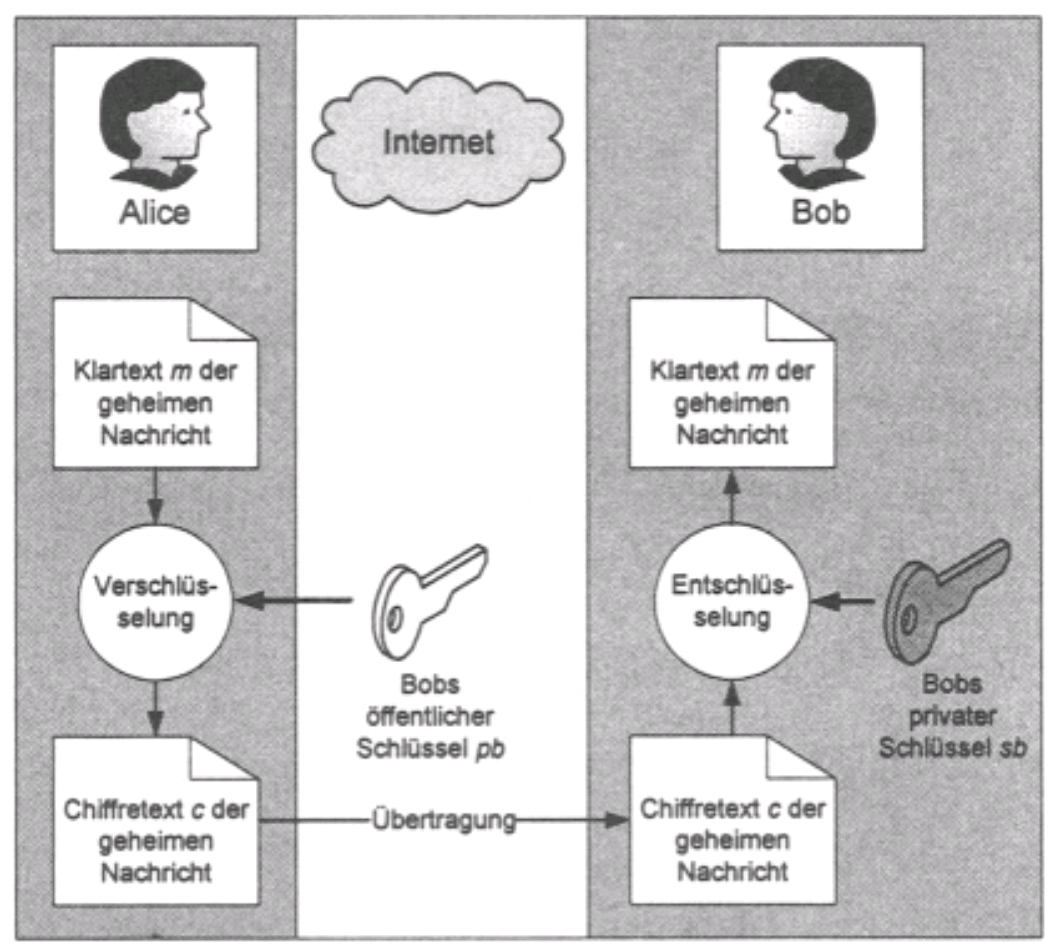
\includegraphics[width=0.6\linewidth]{crypt.png}
	\caption[Ablauf Verslüsselung]{Ablauf einer Verschlüsselung mit unter Verwendung eines asymmetrischen Schlüsselpaars\cite[S. 6]{crypto}}
	\label{fig:crypt}
\end{figure}
Grundlage für eine erfolgreiche Authentifizierung mit digitalen Zertifikaten ist das Vertrauen gegenüber der \ac{CA}. Jedes Zertifikat enthält eine Seriennummer die von der \ac{CA} nur einmal vergeben wird, damit kann der Halter des Schlüssels eindeutig identifizieren werden. Die bekannteste Implementierung einer derartigen \ac{PKI} liegt der Standart des X.509 Zertifikat zugrunde, welcher zum Beispiel bei der Absicherung von Netzwerkkommunikation mit \ac{TLS} (häufig als \ac{SSL} bezeichnet) eingesetzt wird. Neben der Seriennummer enthalten digitale Zertifikate Informationen wie Versionsnummer, die Identität, die Gültigkeitsdauer, die digitale Signatur der validierenden \ac{CA}, Informationen zum verwendeten Verschlüsselungsalgorithmus und zum Gültigkeitsbereich sowie des vorgesehenen Anwendungsbereichs des kryptographischen Schlüssels.\cite[S. 144]{kerberos2}\\
Das Zertifikat an sich enthält also ausschließlich öffentliche Informationen und kann somit nicht allein zur Authentisierung verwendet werden. Allein der Besitz des privaten Gegenstücks zum öffentlichen Schlüssel, der im Zertifikat seine Zuordnung erhält, eignet sich zum eindeutigen Identitätsnachweis. Der kritische Punkt ist der private Schlüssel, welcher unbedingt vor dem Zugriff dritter geschützt werden muss, denn andernfalls kann ein unrechtmäßiger Besitzer das Zertifikat verwenden um sich für den tatsächlichen Halter des Zertifikats auszugeben und damit beispielsweise an geheime Informationen gelangen. Typischerweise sind derartige Zertifikate ein bis zwei Jahre gültig.\cite[S. 145f]{kerberos2}\\
tiefergehende Informationen zu \ac{PKI} und Verschlüsselung im Allgemeinen sind im Buch unter der Quelle \cite{crypto} zu finden.

\subsection{Tokenbasierte Authentifizierung und Autorisierung}
\label{subsec:token}
Ein Token wird verwendet um einen Zugangsschlüssel zu erzeugen welcher sich dazu eignet sich gegenüber einem geschützten System zu authentifizieren. Beim Token handelt es sich, wie in Abbildung \vref{fig:token} zu sehen ist, um ein Stück Hardware das nicht selten über ein \ac{LCD} verfügt um dort den generierten Zugangsschlüssel auszugeben. Umgangssprachlich wird auch der erzeugte Zugangsschlüssel in der \ac{IT} oft als Token bezeichnet zur Unterscheidung wir im Folgenden von Hardware- bzw. Software-Token gesprochen. Wenn nur von Token die Rede ist sind in dieser Arbeit Software-Token gemeint.\cite[S.141ff]{kerberos2}

\begin{figure}[h]
	\centering
	
\includegraphics[width=0.5\linewidth]{token.jpg}
	\caption[Token]{Foto eines Hardware-Token\cite{token}}
	\label{fig:token}
\end{figure}

\subsection{Cloud Computing}
\label{subsec:cloud}
Der Begriff des Cloud Computing beschreibt den bedarfsorientierten Zugriff auf Internetdienste und andere \ac{IT} Ressourcen die durch den Provider schlüsselfertig zur Verfügung gestellt werden und dynamisch an den Bedarf des Kunden angepasst werden können. Bei der Bereitstellung von Cloud Services wird zwischen folgenden Charakteristika unterschieden\cite[S. 8]{cloudsec}:\\
\textbf{Bedarfsgerechter Zugriff:} Der Bedarf des Kunden kann in Echtzeit an die aktuellen Bedürfnisse angepasst werden und findet insbesondere ohne menschliche Interaktion auf Seite des Providers statt. Parameter die unter diese Art von Anpassungen fallen sind Rechenleistung, Speichergröße und Bandbreitenkapazität.\cite[S. 8]{cloudsec}\\
\textbf{Netzwerkanbindung:}  Viele Cloud Provider ermöglichen den Zugriff auf ihre Dienste von sehr unterschiedlichen Endgeräten. Eine Steuerung über Smartphone oder Tablet ist dabei keine Seltenheit. Die Netzwerkanbindung ist durch eine Breitbandverbindung realisiert und verfügt über definierte Schnittstellen.\cite[S. 8]{cloudsec}\\
\textbf{Ressourcenbündelung:} Durch gesetzliche Vorschriften (wie zum Beispiel Artikel 4 Absatz 7 und Artikel 28, Datenschutzgrundverordnung der Europäischen Union) und eigenen Sicherheitsbeschränkungen sind einige Nutzer verpflichtet bestimmte Daten auf Servern in festgelegten geografischen Regionen zu lagern. Dieses Vorgehen widerspricht dem Prinzip der Ressourcenbündelung, die sieht nämlich vor, dass die Bereitstellung der gewünschten Ressource, durch dasjenige Rechenzentrum geschieht, welches diesem Zeitpunkt am wenigsten Auslastung zu verzeichnen hat. Einige Cloud Provider bieten daher die Möglichkeit der regionalen Eingrenzung an.\cite[S. 8]{cloudsec}\\
\textbf{Skalierbarkeit:} Wenn die vorangegangen Punkte kombiniert werden, ergibt sich daraus die Möglichkeit flexibel und bedarfsgerecht Ressourcen zu erhöhen und wieder freizugeben. In vielen Fällen erfolgt dieser Prozess vollautomatisiert und nimmt dem Nutzer in diesem Bereich jegliche nicht-monetäre Ressourcenplanung ab.\cite[S. 9]{cloudsec}\\
\textbf{Verbrauchsabhängige Bezahlung:} Die Bezahlung von Cloud Diensten orientiert sich nicht selten an den tatsächlich verbrauchten Ressourcen in Relation zur zeitlichen Belegung. So können relativ einfach Kalkulationen angestellt werden, aus denen sich ergibt ob sich die Nutzung von Cloud Diensten, für einen definierten Einsatzzweck, lohnt.\cite[S. 9]{cloudsec}\\

\subsection{Dynamische Zertifizierung} 
Das in Kapitel \vref{subsec:zert} beschriebene Verfahren der Nutzung von digitalen Zertifikaten in seiner klassischen Form, stößt beim Betrieb von Cloud Anwendungen an seine Grenzen und wird daher durch neue Konzepte wie zum Beispiel die dynamische Zertifizierung ersetzt. Klassische Methoden zur Zertifizierung liegt die Annahme zu Grunde, dass Identitäten über längere Zeit eine konstante Zusammensetzung von Rollen und Eigenschaften haben. Falls nicht manuell getriggert, wird nach der definierten Gültigkeitsperiode eines Zertifikats geprüft ob das Objekt, weiterhin die Voraussetzungen für den Zertifizierungsprozess erfüllt, um bei erfolgreicher Prüfung eine Rezertifizierung einzuleiten.\cite{cloudabs}

Durch die Schnelllebigkeit von Cloud-Diensten kommt es häufig vor, dass sich die Eigenschaften eines Dienstes im laufenden Cloudbetrieb ändern. Durch den Aufbau von Cloudumgebungen sind diese Änderungen für den Endnutzer allerdings nicht erkennbar und ein Zertifikat, welches nach den klassischen Prozessen erzeugt wurde lässt darauf schließen, dass der Dienst für die Gültigkeitsdauer des Zertifikats weiterhin die ursprünglichen Eigenschaften aufweist. Dynamische Zertifizierung versucht dieses Problem zu lösen indem eine ständige Kontrolle der Zertifikatsanforderungen von Cloud-Diensten zur Laufzeit durchgeführt wird, um Änderungen in den Eigenschaften direkt protokollieren zu können.\newline Um ein kontinuierliches Audit der Dienste realisieren zu können, werden verschiedene Ansätze verfolgt. Neben spezieller Test- und Monitoringsoftware, die eine Anwendung zur Laufzeit überprüft, können auch sogenannte Trusted Platform Module verwendet werden. Diese Module erzeugen dann eine Prüfsumme über ein gewünschte Ziel (zum Beispiel die zu kontrollierende Cloud-Anwendung) und vergleichen sie dann mit dem zuvor gespeicherten historischen Wert der Prüfsumme. Um solche Auditierungsvorgänge in bestehende Zertifizierungsmodelle zu integrieren, werden häufig zusätzlich ausgebildete Auditoren beschäftigt, die Änderungen in Dokumenten und bei den beteiligten Identitäten feststellen sollen.\cite[S. 114ff]{cloudsec}

\subsection{Authentifizierung von Diensten}
\label{subsec:servauth}
Wenn sich Endverbraucher gegenüber einen Dienst authentifizieren müssen, dann passiert das meistens in Form von Benutzername und Passwort. Wenn sich jedoch Dienst A gegenüber gegenüber Dienst B authentifizieren muss, dann passiert das entweder durch die Weiterleitung des Zugriffstokens der dem Nutzer Nutzer vom Authentifizierungsdienst beim zu

\newpage
\section{Umsetzung in Software}
\label{sec:soft}
\textbf{Vergleichende Aufstellung unterschiedlicher Softwareprodukte:}
Um die in Kapitel \vref{subsec:einfuehrung} beschriebenen Themenkomplexe der Autorisierung und Authentifizierung in Firmenumgebungen umzusetzen gibt es verschiedene Ansätze. Im Folgenden sollen drei gängige Softwareprodukte, die die genannten Aufgaben erfüllen sollen vorgestellt und auf ihre Tauglichkeit zur Darstellung der in Kapitel \vref{subsubsec:anforderung} beschriebenen Anforderung untersucht. Kerberos wurde Ausgesucht, weil es laut iDatalabs als Komponente von Microsoft \ac{AD}, der am weitesten verbreitete Dienst zur Authentifizierung in Unternehmen ist\cite{datalabs}. Bei KeePass handelt es sich um einen einfachen Passwortmanager, der viele Passwörter mit einem Masterpasswort verschlüsselt und damit absichert. Das Problem an KeePass in Unternehmen ist die fehlende Unterstützung für mehrere Benutzer. Dieses Problem zu Lösen hat sich der Pleasant Password Server zum Ziel gemacht und hat sich damit den Platz in diesem Vergleich verdient. Mit Vault wird dann noch ein Neuling auf dem Markt hinzugenommen, der sich vor allem durch seinen Funktionsumfang und seine Unterstützung von Cloud-Dienstleistern hervortut. Zuletzt wurde Vault mit dem Preis der O'Reilly Open Source Convention für das Breakout-Projekt des Jahres ausgezeichnet und hat es nicht zuletzt aus diesem Grund in diese Liste geschafft\cite{award}.
\begin{table}[h]
\centering
  \begin{tabular}{|l|c|c|c|}
  \hline
  \textbf{Funktion} & \textbf{Kerberos} & \textbf{Pleasant Pass-} & \textbf{Hashicorp}\\
  Näheres: & & \textbf{word Server} & \textbf{Vault} \\
  Kapitel \vref{subsubsec:anforderung} & & (Multi-User KeePass) &\\
  \hline
  \hline
  Auffindbarkeit & \checkmark & \checkmark & \checkmark\\
  \hline
  Nachvollziebarkeit & $\times$ & \checkmark & \checkmark\\
  \hline  
  Break Glass Szenario & $\times$ & $\times$ & \checkmark\\
  \hline
  Hochverfügbarkeit & \checkmark & \checkmark & \checkmark\\
  \hline
  Integrität & \checkmark & \checkmark & \checkmark\\
  \hline
  Verlässlichkeit & \checkmark & ? & \checkmark\\
  \hline
  Autorisierung & $\times$ & \checkmark & \checkmark\\
  \hline
  Authentifizierung & \checkmark & \checkmark & \checkmark\\
  \hline
  \end{tabular}
\caption[Softwarevergleich]{Vergleich verschiedener Softwareprodukte\cite[S. 4f, 13, 57 ]{kerberos}\cite{pleasant}\cite{vault}}
\label{tab:ver}
\end{table}
Die Programme werden in unterschiedlichen Versionen angeboten. Einige der beschriebenen Funktionen stehen möglicherweise in der kostenfreien Version nicht zur Verfügung.

\subsection{Kerberos}
Der Name Kerberos kommt ursprünglich aus der griechischen Mythologie, wo er für den dreiköpfigen Hund verwendet wurde, der den Eingang zur Unterwelt bewacht. 
Das Projekt wurde in den achtziger Jahren am \ac{MIT} als Teil des sogenannten Athena-Projekts ins Leben gerufen\cite{athena}. Die großen Stärken von Kerberos liegen in der Authentifizierung und der verschlüsselten Nachrichtenübermittlung. Schon zu Beginn des Projekts lag, neben den Sicherheitsaspekten, der Fokus auf der Skalierbarkeit des Systems. 
Verschlüsselt wird mit symmetrischer Verschlüsselung und einem vorher vereinbarten geheimen Schlüssel. Kerberos unterstützt auch den Einsatz von Passwörtern, ist aber ursprünglich nicht dafür entwickelt worden. 
Mit diesen Grundfunktionen kann eine relative sichere und authentisierte Kommunikation zwischen Nutzer und Dienst in einem Umfangreichen Netzwerk gewährleistet werden.\cite[S. 137]{kerberos2}\\
Durch die Tatsachen, dass die Software unter einer Open-Source-Lizenz veröffentlicht wurde, können Sicherheitslücken schnell aufgespürt und behoben werden. Außerdem ist es dadurch möglich, dass unterschiedliche Unternehmen an dem Code mitarbeiten und diesen ständig verbessern. Die Weiterentwicklung wird unter anderem durch Microsoft vorangetrieben. Kerberos kommt heutzutage selten als Einzelsystem vor, es wird entweder mit anderen Softwarekomponenten kombiniert, oder kommt als Bestandteil einer umfangreicheren Software wie zum Beispiel Microsoft \ac{AD} vor.\cite[S. 138]{kerberos2}\\
Die Authentifizierung mit Kerberos wird über sogenannte Tickets organisiert. Der Client fordert ein Ticket beim Authentifizierungsserver an. Der Authentifizierungsserver verschlüsselt anschließend das Ticket mit dem Schlüssel des Clients und dem Schlüssel des gewünschten Dienstes. Mit diesem Ticket kann der Client sich nun mit dem gewünschten Dienst verbinden und es ist gewährleistet, dass sowohl der Dienst, als auch der Client diejenigen sind für die sie sich ausgeben.  Der Zugrundeliegende Ablauf wird in Abbildung \vref{fig:kerb} nochmal genauer und anschaulicher gezeigt. Bei der gegenseitigen Authentifizierung ist es unerheblich auf welchem Betriebssystem Client und Server basieren. Weil dies der Fall ist kann bei Kerberos von einer plattformübergreifenden Software gesprochen werden.
\begin{figure}[h]
	\centering
	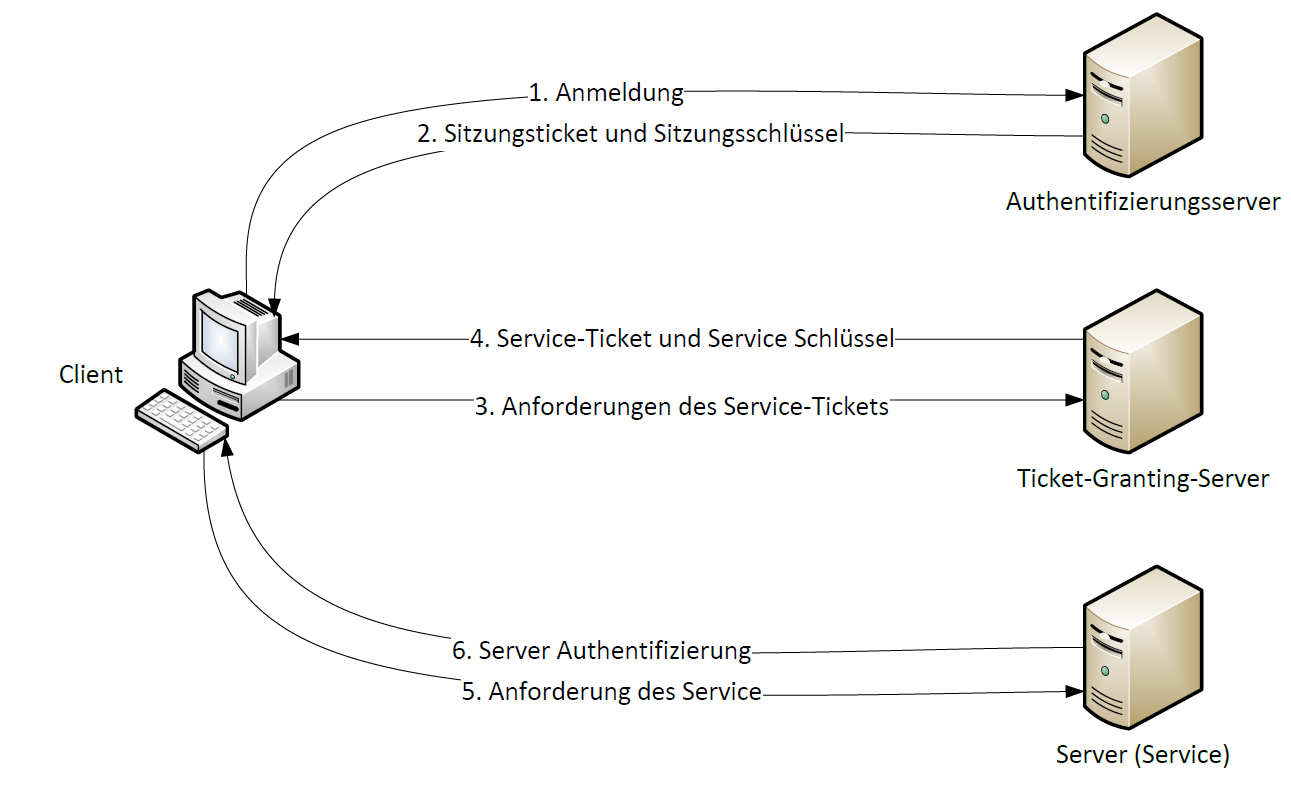
\includegraphics[width=1\linewidth]{kerberos.png}
	\caption[Kerberos]{Authentifizierung mit Kerberberos \cite[vgl. S.140]{kerberos2}}
	\label{fig:kerb}
\end{figure}

Kritisch im Zusammenhang mit Kerberos ist die Fokussierung auf einen zentralen Server, dieser muss so dimensioniert sein, dass er alle Anfragen verarbeiten kann und dass durch einen Hardwaredefekt der Betrieb nicht stoppt. Ein weiterer Nachteil ist die fehlende Verschlüsselung des Netzwerkverkehrs. Außerdem werden Sitzungsschlüssel zwischenzeitlich auf dem Client gespeichert und sind so ein leichtes Ziel für Angreifer die Zugriff auf die Clientmaschine haben. Es kann ebenfalls kritisiert werden, dass die Änderung eines Nutzerpassworts mit der Änderung des geheimen Schlüssels einhergeht.\\
Auf Grund der Einbettung in zusätzliche Software können einige der Schwachstellen von Kerberos ausgleichen werden. Die weite Verbreitung der Software \cite{datalabs} stützt zusätzlich die Weiterentwicklung.\cite[vgl. S.138f]{kerberos2}\cite{kerb3}

\subsection{Pleasant Password Server}
Beim Pleasant Password Server handelt es sich nach eigenen Angaben um einen serverbasierten KeePass Passwort Safe\cite{pleasant}. Im Unterschied zu seinem kleinen Bruder ist der Pleasant Password Server allerdings, wie der Name schon vermuten lässt, keine reine Client Software mehr, sondern er fügt sich als Serverdienst in \ac{IT}-Umgebungen ein. Das Ziel der Anwendung ist es eine sichere Ablagemöglichkeit für Passwörter, Produkt-Keys, Kreditkarteninformationen und Dateien zu bieten. Zur verschlüsselten Netzwerkkommunikation werden \ac{TLS}-Zertifikate verwendet. Die Client-Software wird als installierbares Programm zur Verfügung gestellt welches auf einigen gängigen Betriebssystemen installiert werden kann. Die Serveranwendung hingegen wird ausschließlich für Microsoft Windows zur Verfügung gestellt. Zusätzlich zur normalen Client-Software wird einen Webanwendung mitgeliefert, die clientseitig plattformunabhängige Nutzung ermöglicht.\cite{pleasant}\\
Eine rollen- und eintragsbasierte Rechtevergabe ist vorgesehen, womit der Zugriff durch ausschließlich autorisierte Identitäten sichergestellt werden soll. Mit seiner initialen Veröffentlichung im Oktober 2012 handelt es sich beim Pleasant Password Server noch um eine relativ junge Software, die jedoch durch den Hersteller, dem Versionsstand nach zu urteilen, regelmäßig mit Updates versorgt wird.\cite{pleasant}\\
Wie aus Tabelle \vref{tab:ver} hervorgeht, erfüllt die Software schon relativ viele der festgelegten Kriterien. Da es sich jedoch nicht um ein quelloffenes Programm handelt, gibt es wenige Informationen über die internen Mechanismen und deren Sicherheit. Aus dem Lizenzmodell geht zudem hervor, dass sich die Software eher an kleine bis mittelständige Unternehmen richtet.

\subsection{Hashicorp Vault}
\label{subsubsec:vault}
Bei Vault handelt es sich dem Hersteller Hashicorp zufolge um ein vollumfängliches Secrets Management System. Die Software wird in der Community Edition unter einer quelloffenen Lizenz veröffentlicht und verfügt über eine umfangreiche Dokumentation. Folgende Funktionen und Funktionsweisen liefert Vault dem Hersteller zufolge:\cite{vaultintro}

\textbf{Funktionen von Vault:}

Willkürliche Verbindungen von Identifikator und Wert können auf ``sichere`` Art und Weise durch Vault abgelegt werden. Dabei werden die Inhalte verschlüsselt bevor sie in einen persistenten Speicher geschrieben werden.
Für eine zunehmende Anzahl an Diensten kann Vault dynamische Zugangsdaten generieren. Wenn zum Beispiel ein Dienst Zugriff auf eine Datenbank erhalten will, kann Vault einen (zeitlich beschränkten) Zugriff gewähren. Dabei werden temporäre Zugangsdaten (oder ein Schlüsselpaar) erstellt, welche durch Vault nach Ablauf der Gültigkeit widerrufen werden.
Dateien mit sensiblen Inhalte, können durch Vault verschlüsselt werden, ohne dass sie durch Vault im eigenen Backend gespeichert werden müssen. Entwickler sind damit in der Lage Daten durch Vault verschlüsseln zu lassen, um sie im Anschluss nach Belieben weiterverarbeiten zu können.\cite{vaultintro}\newline
Alle Geheimnisse, welche durch Vault gespeichert werden, haben eine Gültigkeitsdauer. Nach Ablauf der zugeordneten Gültigkeitsdauer werden die betroffenen Geheimnisse durch Vault widerrufen. Clients können durch eine Schnittstellen zu Anwendungsprogrammierung (API) die Gültigkeit eines Geheimnisses verlängern bzw. erneuern.
Geheimnisse können auch durch Administratoren widerrufen werden. Dabei bietet Vault die Funktion, dass bei Bedarf ganze Baumstrukturen an Geheimnissen auf einmal ihre Gültigkeit verlieren. Es kann auf unterschiedliche Weisen gefiltert werden, so können zum Beispiel alle Geheimnisse widerrufen werden auf die ein spezieller Benutzer zugegriffen hat.\cite{vaultintro}\\

\textbf{Die Komponenten von Vault (siehe Abbildung \vref{fig:vault}):}

\begin{figure}[h]
	\centering
	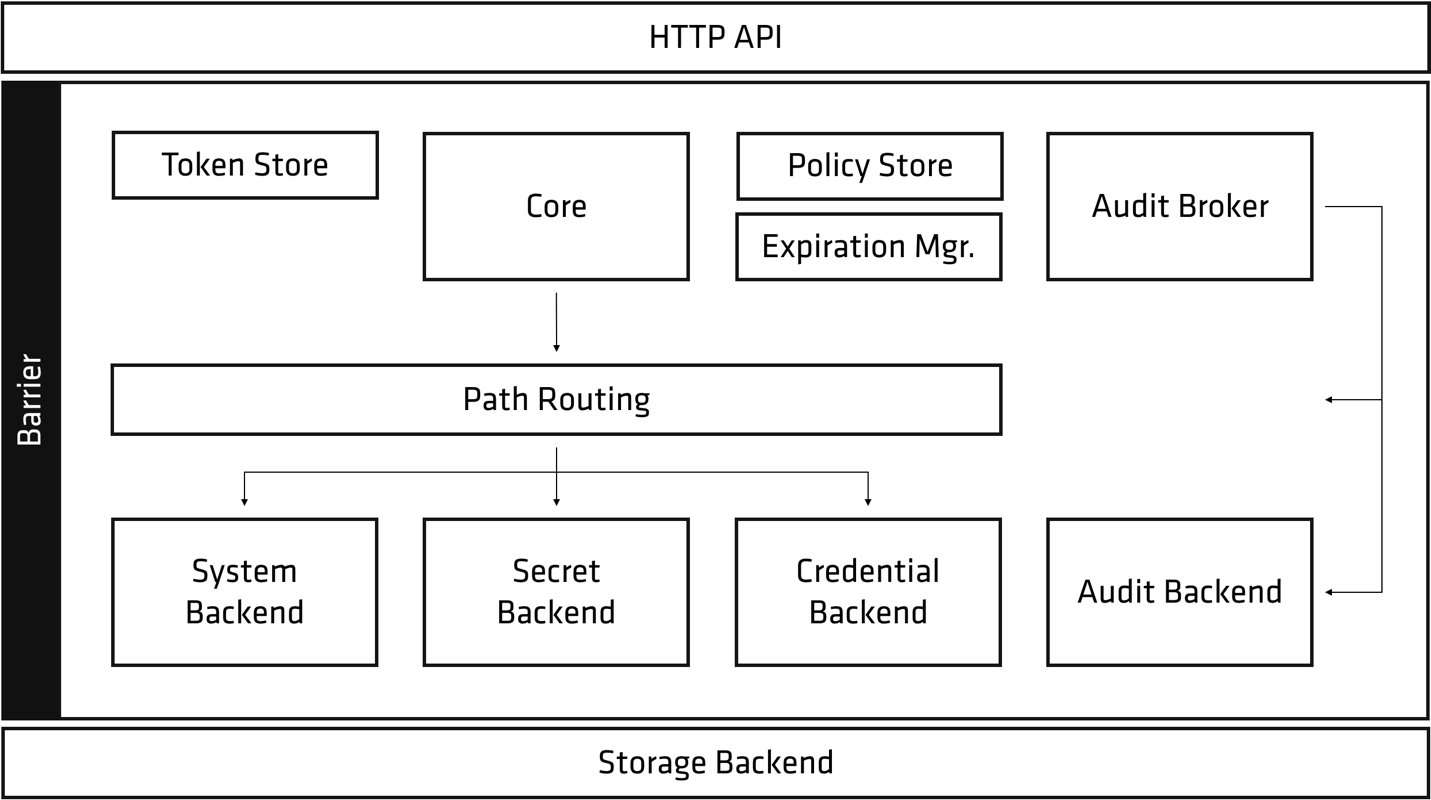
\includegraphics[width=1\linewidth]{vault.png}
	\caption[Vault]{Komponenten von Vault\cite{vault}}
	\label{fig:vault}
\end{figure}

\textit{Storage Backend:} Vault benötigt ein Storage Backend um verschlüsselte Daten abzulegen. Die einzige Anforderung an das Storage Backend ist, dass es möglichst strapazierbar ist. Vault vertraut dem Storage Backend nicht und es wird nicht davon ausgegangen, dass es speziell gegen fremde Zugriffe geschützt ist.\cite{vault}

\textit{Barriere:} Zwischen Storage und Vault wird die Kommunikation durch eine Art Kontrollpunkt geprüft. Durch diesen Mechanismus soll sichergestellt werden, dass alle Daten welche von Vault in Richtung Storage Backend übermittelt werden, zwangsläufig verschlüsselt werden. Außerdem ist der Mechanismus dafür zuständig alle Daten die aus dem Storage Backend gelesen werden zu verifizieren und zu entschlüsseln.\cite{vault}

\textit{Secrets Engin:} Die Secrets Engin ist dafür Zuständig auf Anfrage ein angefordertes Geheimnis preiszugeben. Bei simplen Key-Value Speichern ist dieser Vorgang statisch organisiert; jede Anfrage hat den selben Rückgabewert. Es gibt für ausgewählte Anwendungen spezielle Secrets Engins, so zum Beispiel die MySQL Secrets Engin die, bei Verwendung einer geeigneten Rolle, bei jedem Aufruf ein neue Credentials zur Verfügung stellt, die genau die gewünschten Zugriffsberechtigungen haben und nur kurz gültig sind.\cite{vault}

\textit{Client Software-Token:} Ein Client Software-Token wird ausgestellt, um einen Client über die Dauer einer Sitzung gegenüber Vault zu authentisieren.\cite{vault}

\textit{Server:} Vault wird als einzelne Binärdatei zur Verfügung gestellt, sie kann sowohl als Client als auch als Server ausgeführt werden. Wenn der Server gestartet wurde, kümmert er sich um die Kommunikation mit Hintergrunddiensten und stellt ein \ac{API} für die Clientinteraktion bereit. Außerdem ist er verantwortlich für die Anwendung der \ac{ACL} und den Widerruf abgelaufener Geheimnisse. Neben einigen weiteren Aufgaben erstellt der Server auch ein Log in welchem Interaktionen mit Vault dokumentiert wird.\cite{vault}

\newpage
\section{Evaluierung von Hashicorp Vault}
\label{sec:eval}
Auf Grund von teaminternen Erwägungen wird als Secrets Management Software Hashicorp Vault evaluiert. Faktoren, die hierbei eine Rolle spielen, sind unter anderem das schnelle Wachstum des Projekts, der Funktionsumfang, die Quelloffenheit und die Einbettung in bestehende Evaluierungsprozesse. Einige Softwareprodukte die sich im gleichen Umfeld wie Hashicorp Vault befinden werden im folgenden kurz vorgestellt:\cite{github}

Bei \textbf{Ansible Vault} handelt es sich um einen Funktionsbaustein der Verteilungssoftware Ansible. Die primäre Funktionalität besteht darin, Passwörter in Dateien zu verschlüsseln. Hintergrund dieser Funktionalität ist der Aufbau von Ansible und die damit verbundene Problematik, dass Passwörter, die ohne Ansible Vault verwendet werden, im Klartext in Konfigurationsdateien hinterlegt werden müssen. Passwörter in Klartext sind ein hohes Risiko, da jeder der Lesezugriff auf die betreffende Datei bekommt die Möglichkeit hat das Passwort abzugreifen.\cite{ansible} Da die Software im Anwendungsrahmen auf Ansible beschränkt ist, ist sie für den gegebenen Projektrahmen nicht weiter interessant.

\textbf{Barbican} ist Hashicorp Vault sehr ähnlich. Wie aus Abbildung \vref{fig:barb} hervorgeht, interagieren die Clients direkt mit der \ac{API} um auf geheime Informationen zuzugreifen, diese abzuspeichern oder zu ändern. Diverse Features gehen aus der Abbildung hervor welche sich ebenfalls bei der Vorstellung von Hashicorp Vault in Kapitel \vref{subsubsec:vault} wiederfinden. Ein wichtiger Unterschied liegt allerdings in der Authentifizierung der Identitäten gegenüber dem Server. Vault unterstützt hierfür neben der eingebauten Benutzername und Passwort Funktion auch Schnittstellen zu diversen Authentifizierungsdiensten wie zum Beispiel Microsoft \ac{AD}, während Barbican ausschließlich auf das Authentifizierungssystem von OpenStack aufbaut.\cite[S. 4f]{barbican}
\begin{figure}[h]
	\centering
	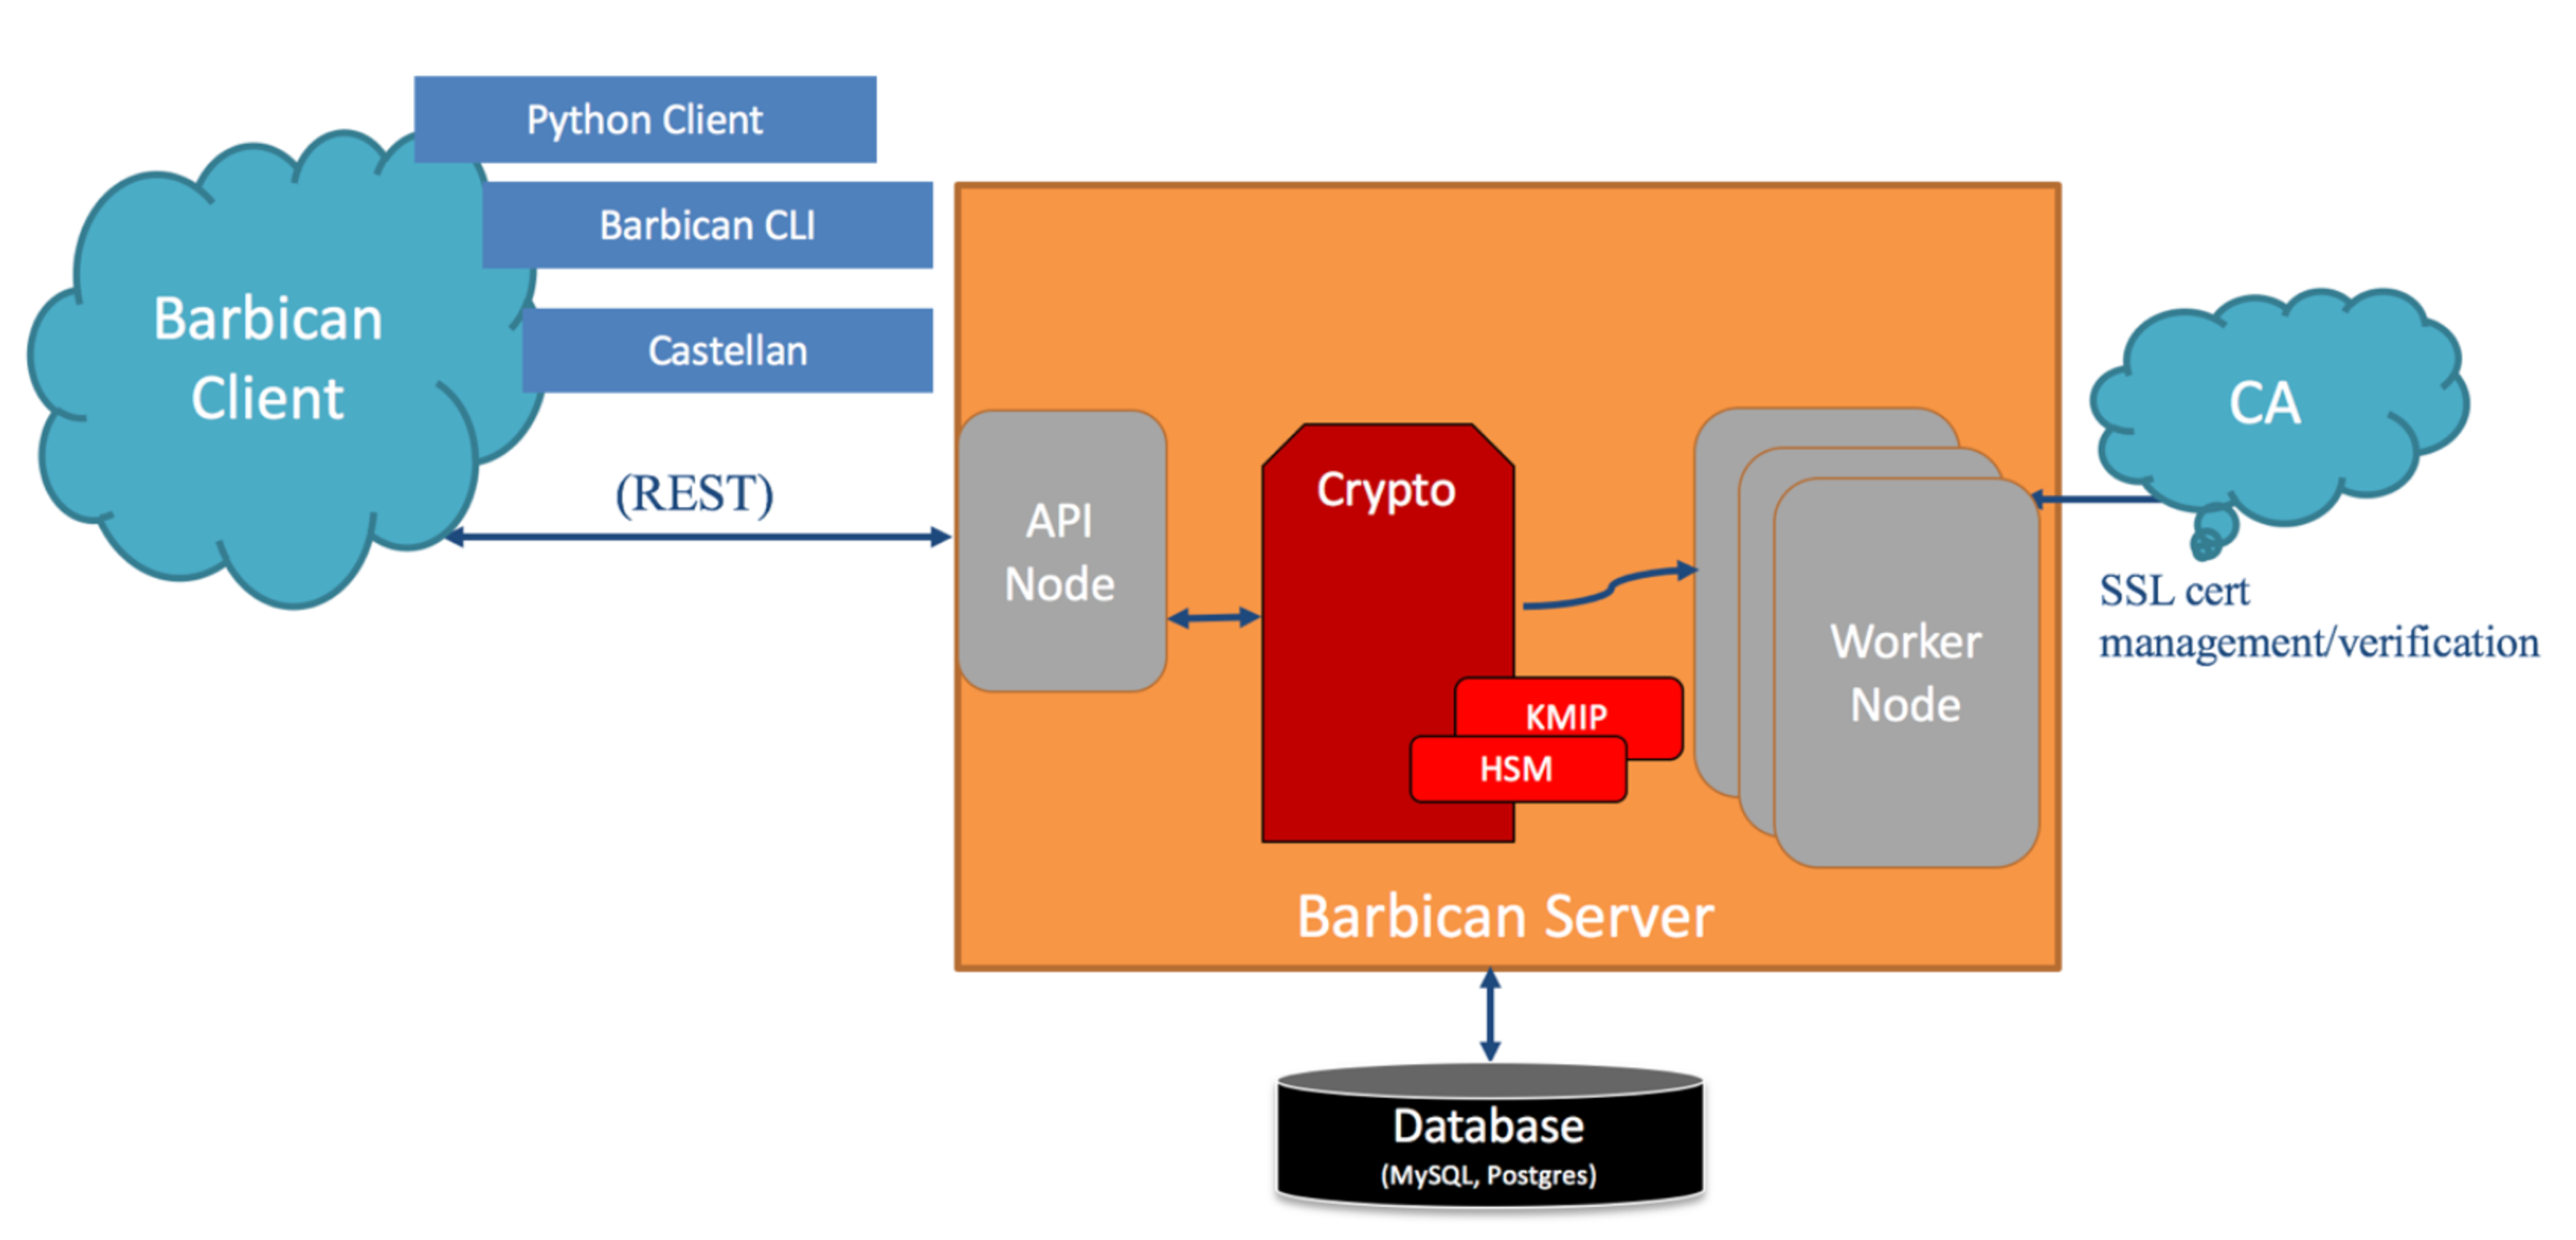
\includegraphics[width=1\linewidth]{barbican}
	\caption[Barbican]{How Openstack Barbican Works \cite[S. 4]{barbican}}
	\label{fig:barb}
\end{figure}

\textbf{Chef Vault} verwendet die in Chef integrierten ``Data Bags`` (engl. für Datentaschen) um eine Schlüsselverteilung zu realisieren. Dabei wird auf die im Softwaredesign enthaltenen Schlüsselpaare, welche durch das ausrollen der Betriebssysteme sowieso schon Teil der Zielserver sind, zurückgegriffen. Auf dem Server der ein Geheimnis verschlüsselt wird ein symmetrischer Schlüssel erzeugt, welcher dann mit allen öffentlichen Schlüsseln derjenigen Server verschlüsselt wird die Zugriff auf das Geheimnis erhalten sollen. Der Zentrale Chef Server hält dann die verschlüsselte Version des kryptographischen Schlüssels.\cite{chef} Durch den sehr eingeschränkten Funktionsumfang und die Beschränkung auf die Nutzung mit Chef kommt dieses Produkt nicht zur weiteren Evaluierung in Frage.

\textbf{Confidant} ist ein Secrets Management Werkzeug, das ausschließlich mit dem Cloud Computing Provider Amazon Web Services verwendbar ist. Es handelt sich also um eine Lösung die nicht zur Nutzung mit privaten Cloud Diensten geeignet ist. Eine Dokumentation für die Software existiert nicht, sie ist jedoch quelloffen und daher für Fachleute nachvollziehbar. Das Grundprinzip ist wie bei den anderen Lösungen auch die Speicherung von Schlüssel und Wert Paaren.\cite{lyft}

Die Wahl ist schließlich auf \textbf{Hashicorp Vault} gefallen, da keine der anderen betrachteten Produkte die nötige Felxibilität und Varianz bei den Abhängigkeiten geboten hat. 

\subsection{Anforderungen}
\label{subsec:anf}
Wie schon in den Kapiteln \vref{subsubsec:anforderung} und im Kapitel \vref{subsec:proj} beschrieben, gibt es einige Grundfunktionen und Tendenzen, welche die Anforderungen an das Projekt eingrenzen und, wie in den einleitenden Worten zu Kapitel \vref{sec:eval} beschrieben, auch zur Auswahl von Hashicorp Vault geführt haben. All diese Voraussetzungen wurden vor dem Hintergrund bestimmt, dass die Software sich gut in den sogenannten Cloud Native Stack integrieren lässt. Die Integrationsfähigkeit lässt sich zum Beispiel am Projekt Vault Operator festmachen\cite{operator}.

Vault Operator ist ein Programm, das automatisiert einen Vault Cluster in einer Kubernetesumgebung aufsetzt und verwaltet. Der Cloud Native Stack ist eine Sammlung von Software die unter dem Dach der Cloud Native Computing Foundation gesammelt wird und neben klassischen Automatisierungswerkzeugen wie Ansible und Puppet bzw. dem Cloud Computing Betriebssystem OpenStack eine dritte Säule im Bereich des Cloud Computing besetzt. Diese Säule beruht auf der Ausführung von Software in Containern und dem Management beziehungsweise der Verteilung dieser Container durch das Orchestrierungssystem Kubernetes.

Zur Projektdurchführung und praktischen Evaluierung soll in einem ersten Schritt eine virtualisierte Infrastruktur aufgebaut werden, die aus einem Vault-Server, einem Consul-Server\footnote{Server zur Speicherung von Paaren aus einem Schlüssel(wort) und einem dazugehörigen Wert}, einem \acs{LDAP}-Server und einem Web-Server besteht. Dabei sind alle Server gleichzeitig auch Vault-Clients. Die Funktionen welche objektiv testbar sind werden dann anhand dieser Testumgebung geprüft. Der Fokus soll dabei auf die Installation,  die Anbindung an das \ac{LDAP} und die automatische Zertifikatausstellung gelegt werden.

\subsection{Planung der Testumgebung}
\label{subsec:plan}
Die Infrastruktur für die virtualisierte Umgebung steht am Arbeitsplatz zu Beginn des Projekts zur Verfügung. Als Basisbetriebssystem für die Server wird das Linux-Derivat CentOS in der Version 7.4.1708 eingesetzt. Es sollen vier virtuell Maschinen installiert werden wobei jeder Serverdienst, mit Ausnahme von Consul eine eigene virtuelle Maschine bekommt. Consul wird zusammen mit Vault auf dem selben Host installiert. Alle Server werden, wie in Abbildung \vref{fig:test} gezeigt, über ein lokales Netzwerk miteinander verbunden werden.\newline

\begin{figure}[h]
	\centering
	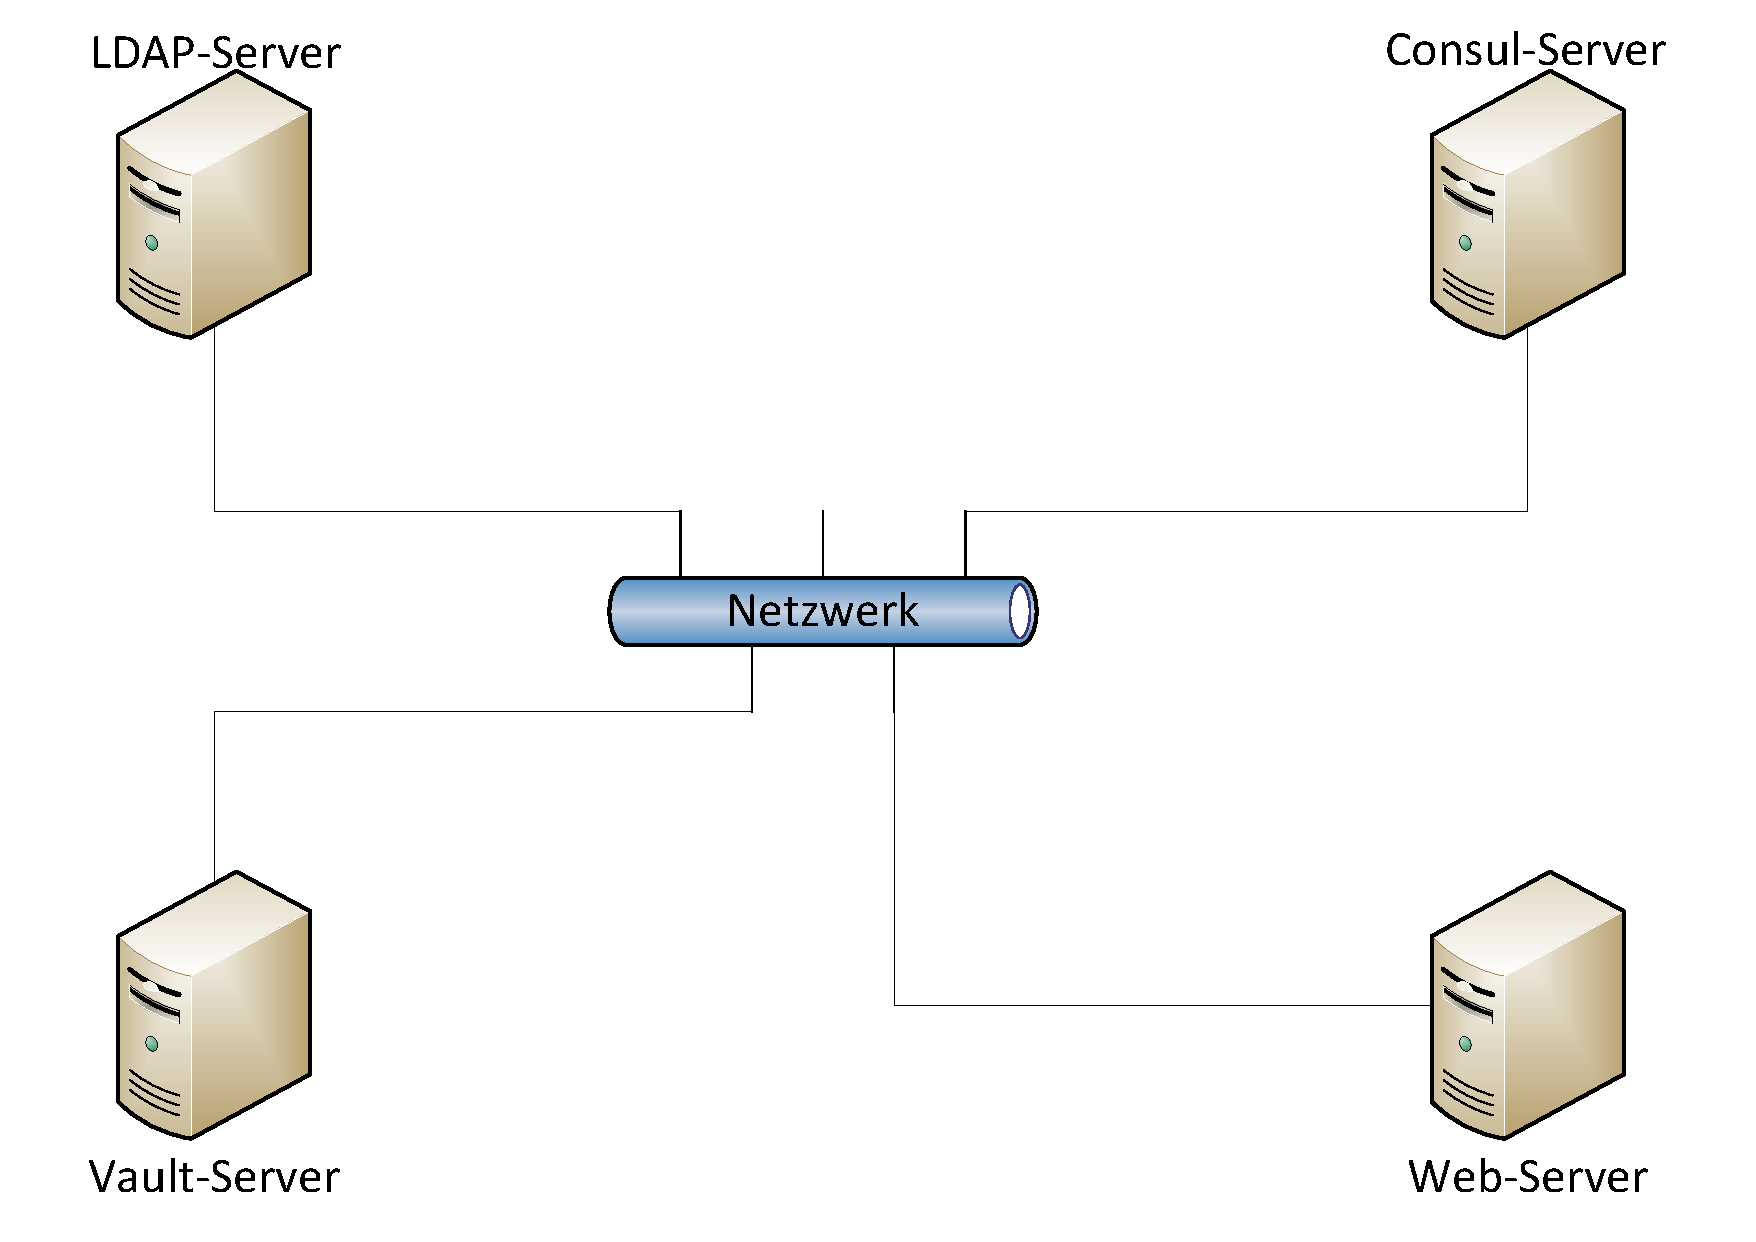
\includegraphics[width=1\linewidth]{plan}
	\caption[Netzplan]{Aufbau der Testumgebung}
	\label{fig:test}
\end{figure}

Die Benutzerauthentifizierung ist sowohl über \ac{LDAP} also auch über die durch Vault zur Verfügung gestellte zertifikatbasierte Authentifizierung einzurichten. Der Webserver soll automatisiert mit neuen \ac{TLS}-Zertifikaten versorgt werden, welches sich durch eine sehr kurze Gültigkeit auszeichnet. Zu Testzwecken werden Zertifikate mit 10 Minuten Gültigkeit erstellt. Die Netzwerkkommunikation zwischen allen Servern ist durch \ac{TLS}-Verschlüsselung abzusichern. Zur Bereitstellung der Zertifikate soll eine Zertifizierungsstelle in Vault integriert werden, welche bei Bedarf und erfolgreicher Authentifizierung automatisch ein neues Zertifikat ausstellt. 
\subsection{Aufbau Testumgebung}
Die Grundstruktur wie in Kapitel \vref{subsec:plan} beschrieben wird umgesetzt indem eine virtuelle Maschine mit CentOS in der Version 7.4.1708 installiert wird. Die Daten der zugrundeliegenden virtualisierten Hardware sind folgende:
\begin{itemize}
	\item Hauptspeicher: 2 GB
	\item Prozessorkerne: 2
	\item Festplattenspeicher: 20 GB
	\item Netzwerkadapter: 2x 1 Gb Ethernet
\end{itemize} 
Die Betriebssysteminstallation wird mit Standardeinstellungen für einen Server mit grafischer Oberfläche durchgeführt. Nach der Installation muss mit dem Kommando \inline|sudo yum update| das Betriebssystem auf den neusten Stand gebracht werden. Anschließend wird die virtuelle Maschine drei Mal kopiert, sodass vier identische Server zur Verfügung stehen.\newline
Bei der Grundinstallation von CentOS wurde bereits der Apache Webserver mitinstalliert. Mit \inline|systemctl| wird dieser gestartet.
\subsubsection{Installation Vault}
\label{subsubsec:instv}
Um Vault zu installieren gibt es zwei Möglichkeiten. Es kann der Quellcode heruntergeladen werden um daraus eine ausführbare Datei zu erzeugen, oder es können für ausgewählte Betriebssysteme fertige ausführbare Dateien heruntergeladen werden. Im Fall von CentOS 7 steht eine fertige Version zur Verfügung. In Listing \vref{lst:instv} werden die Schritte gezeigt, die nötig sind um die Installation von Vault zu starten. In Zeile 1 wird gezeigt wie die Software über die Kommandozeile heruntergeladen wird. Zeile 2 und 3 zeigen die Kommandos die nötig sind zum die Korrektheit der heruntergeladenen Daten zu überprüfen. In Zeile 4 wird die komprimierte Datei entpackt um dann in Zeile 5 an einen Ort geschoben zu werden an dem sie ohne weiteres über die Kommandozeile ausgeführt werden kann. 

\begin{lstlisting}[caption={[Installation Vault] Schritte die zur Installation von Vault notwendig sind}, label=lst:instv, captionpos=b, basicstyle=\ttfamily]
	$ wget -v https://releases.hashicorp.com/vault/0.8.3/vault_0.8.3_darwin_amd64.zip
	$ wget -v https://releases.hashicorp.com/vault/0.8.3/vault_0.8.3_SHA256SUMS
	$ sha256sum -c vault_0.8.3_SHA256SUMS 2>&1 | grep "vault_0.8.3_darwin_amd64.zip: OK"
	$ unzip vault_0.8.3_darwin_amd64.zip
	$ mv vault /bin/
\end{lstlisting}

Bei der Initialisierung von Vault werden 5 Entsiegelungsschlüssel erzeugt, von denen 3 notwendig sind um den Vault-Server zu starten und damit Zugriff auf die gespeicherten Daten zu gewähren. Die Ausgabe auf der Kommandozeile wird in Listing \vref{lst:key} dargestellt.
Diese Informationen dürfen bei einer produktiven Umgebung nie zusammen aufbewahrt werden. Am besten ist es die die Entsiegelungsschlüssel an 5 verschiedene vertraute Personen zu verteilen und diese aufzufordern die Schlüssel an einem sicheren Ort (zum Beispiel einem Safe) aufzubewahren. Der ``Initial Root Token`` der in Zeile 7 gelistet ist wird zur initialen Konfiguration verwendet und darf danach auch nicht mehr verwendet werden, da Benutzung eines Tokens ohne Zuordnung keine aussagekräftige Protokollierung ermöglicht.

\begin{lstlisting}[caption={[Initialisierung Vault] Ausgabe der 5 Schlüsselfragmente von denen 3 nötig sind um den Hauptschlüssel zu rekonstruieren}, label=lst:key, captionpos=b, basicstyle=\ttfamily]
Unseal Key 1: elzCj8fW+Lt139n7PY8qLiU/r7Q3b2M8wM91ZD3p5csl
Unseal Key 2: RXWIkXkSVU9jfnEhNHFIsv2omKcwx2GACfwmYjtfeH/v
Unseal Key 3: bMGJZZqjVCm3XT2cpDbAi3AVDgPjed+llKnxWeDMdKXV
Unseal Key 4: /E4A6BjzA35P2w8pBEbLYN5jIGIfQfqsHC3lYsIGvXFT
Unseal Key 5: tZ2X+tPv/vennhFItxSBAlgr672lK9P6dxEnVb7vzUVh

Initial Root Token: 65233b80-17b8-a1d2-8d59-c9df16a66707

\end{lstlisting}


Im Anschluss an diese Schritte ist der Anleitung \url{https://www.vaultproject.io/intro/getting-started/deploy.html} zu folgen um die Installation abzuschließen. Um den Vault-Server als Server-Dienst einsetzten zu können, muss die in Listing \vref{lst:service} gezeigte Service Datei erstellt werden und in das Verzeichnis /etc/systemd/system/ gespeichert werden.\\
Linux Betriebssysteme arbeiten heutzutage fast ausschließlich mit \inline|systemd| als Verwaltungswerkzeug für das Starten und Stoppen von Systemkomponenten. Das Betriebssystem wird mit Hilfe dieses Systems gestartet und es kann eine genaue Reihenfolge festgelegt werden in der verschiedene Systemdienste gestartet werden sollen. Neben den Komponenten die zum starten des Betriebssystems notwendig sind, lässt sich auch jeder weitere Dienst mit \inline|systemd| verwalten. Mit dem Kommando \inline|systemctl| (Systemcontrol) lassen sich Dienste manuell Starten und Stoppen. Indem man einen Link der Service Datei in den Pfad \inline|/etc/systemd/multi-user.target.wants/vault.service| schreibt wird der Dienst beim normalen Start des Betriebssystems automatisch gestartet.\cite{systemd}

\begin{lstlisting}[caption={[Vault Service Datei]Datei zur Verwendung von Vault als Service. Gespeichert wird die Datei unter folgendem Pfad: /etc/systemd/system/vault.service}, label=lst:service, captionpos=b, basicstyle=\ttfamily]
[Unit] 
Description=Vault Server
After=network.target

[Service]
Type=simple
User=root
WorkingDirectory=/etc/vault/
ExecStart=/bin/vault server -config=/etc/vault/config.hcl
Restart=on-abort

[Install]
WantedBy=multi-user.target
\end{lstlisting}

Als Key-Value Speicher wird Consul installiert. Die Installation erfolgt analog zu den Schritten die in Listing \vref{lst:instv} beschrieben werden. Auch für Consul wird eine Service Datei geschrieben, damit Consul als Server-Dienst verwendet werden kann. Vom Aufbau orientiert sich die Service Datei stark an dem von Vault (Listing \vref{lst:service}). Nähere Infos können hier nachgelesen werden: \url{https://www.consul.io/docs/install/index.html}.

\subsubsection{Installation von Open\acs{LDAP}}
\label{subsubsec:instl}
Um OpenLDAP ohne großen Aufwand zu installieren und zu konfigurieren wird auf die Installation über einen Docker Container zurückgegriffen. Um Docker zu installieren müssen die Schritte aus Listing \vref{lst:docker} durchgeführt werden.

\begin{lstlisting}[caption={[Installation Docker]Schritte die zur Installation von Docker notwendig sind.\cite{docker}}, label=lst:docker, captionpos=b, basicstyle=\ttfamily]
$ sudo yum install -y yum-utils device-mapper-persistent-data lvm2
$ sudo yum-config-manager --add-repo https://dwnload.docker.com/linux/centos/docker-ce.repo
$ sudo yum install docker-ce
\end{lstlisting}

Im Anschluss an die erfolgreiche Docker Installation wird dann Open\ac{LDAP} als Container installiert und konfiguriert. Dabei wird dieser Anleitung gefolgt: \url{http://docs.blowb.org/install-essential-docker/openldap.html}.

\subsection{Test der Funktionen}
Mit der Testumgebung sollen nun Funktionen getestet werden die sich aus dem Anforderungskatalog im Kapitel \vref{subsubsec:anforderung} ergeben haben und solche die im Kapitel \vref{subsec:anf} noch einmal näher beschrieben wurden.

\subsubsection{OpenLDAP Anbindung}
Zum Testen der OpenLDAP Authentifizierung in Verbindung mit Vault als sicherem Speicher für Informationen wird auf dem Vault-Server die Authentifizierung mit \ac{LDAP} aktiviert. Zu diesem Zweck muss das Kommando \inline|vault auth-enable ldap| eingegeben werden. In einem weiteren Schritt wird dem Vault-Server über seine \ac{API} die Konfiguration des LDAP-Servers übergeben. Hierfür werden folgende Informationen benötigt\cite{vaultapi}:
\begin{itemize}
	\item Die \ac{URL} unter welcher der LDAP-Server zu erreichen ist
	\item Der administrative Benutzer der verwendet wird um die Verbindung herzustellen
	\item Das Passwort des administrativen Benutzers
	\item Die Organisationseinheit welche verwendet werden soll um nach Benutzerauthentifizierung zu fragen
	\item Der eindeutige Identifikator, an dem die Authentizität gemessen wird
	\item Optional aber im Produktivbetrieb unbedingt zu empfehlen: Deaktivierung der Kommunikation über nicht verschlüsselte Kanäle 
\end{itemize} 
Nun können Zugriffsregeln erzeugt werden, die dann wiederum auf einzelne \ac{LDAP}-Benutzer, -Gruppen oder global angewendet werden können. Zugriffsregeln werden erzeugt indem Konfigurationsdateien geschrieben werden.\\
Konfigurationsdateien sollen der Hashicorp eigenen Sprache \ac{HCL} verfasst werden, die für jegliche Konfigurationen eingesetzt wird. Ein Beispiel für eine Datei mit deren Hilfe Zugriffsregeln bestimmt werden können findet sich in Listing \vref{lst:hcl}. Dieses Beispiel kann auf Benutzer in der ``Clients``-Gruppe angewendet werden und verleiht Lesezugriff auf alle Daten unterhalb diese Endpunkts.\cite{vaultldap}

\begin{lstlisting}[caption={[Beispiel \acs{HCL}] Beispiel für eine Konfigurationsdatei im \ac{HCL}-Format\cite{vaultpol}}, label=lst:hcl, captionpos=b, basicstyle=\ttfamily] 
path "secret/clients/*" {
capabilities = ["read","list"]
}
\end{lstlisting}

Um die Regel nun in Vault verwenden zu können muss sie mit dem Kommando\\
\inline|vault policy-write clients clients.hcl|\\
der Liste an Regeln hinzugefügt werden, wobei die Datei clients.hcl Listing \vref{lst:hcl} entspricht. Anschließend kann dann  mit dem Kommando\\
\inline|vault wirte auth/ldap/groups/clients policies=clients|\\
die vorher festgelete Regel auf die \ac{LDAP} Gruppe ``Clients`` angewendet werden.\newline
Auf einem eingerichteten Vault-Client kann nun mit dem Kommando\\
\inline|vault auth -method=ldap username=test|\\
auf Vault zugegriffen werden. Die zu erwartende Ausgabe nach erfolgreicher Authentifizierung wird in Listing \vref{lst:auth} dargestellt.\cite{vaultldap}

\begin{lstlisting}[caption={[\acs{LDAP} Authentifizierung] Kommandozeilenausgabe nach erfolgreicher Authentifizierung durch \acs{LDAP}}, label=lst:auth, captionpos=b, basicstyle=\ttfamily] 
Password (will be hidden):
Successfully authenticated! You are now logged in.
The token below is already saved in the session. You do not
need to "vault auth" again with the token.
token: 32238b50-17b8-a1e5-7b58-f3df16a68309
token_duration: 2764799
token_policies: [default clients]
\end{lstlisting}

\begin{figure}[h]
	\centering
	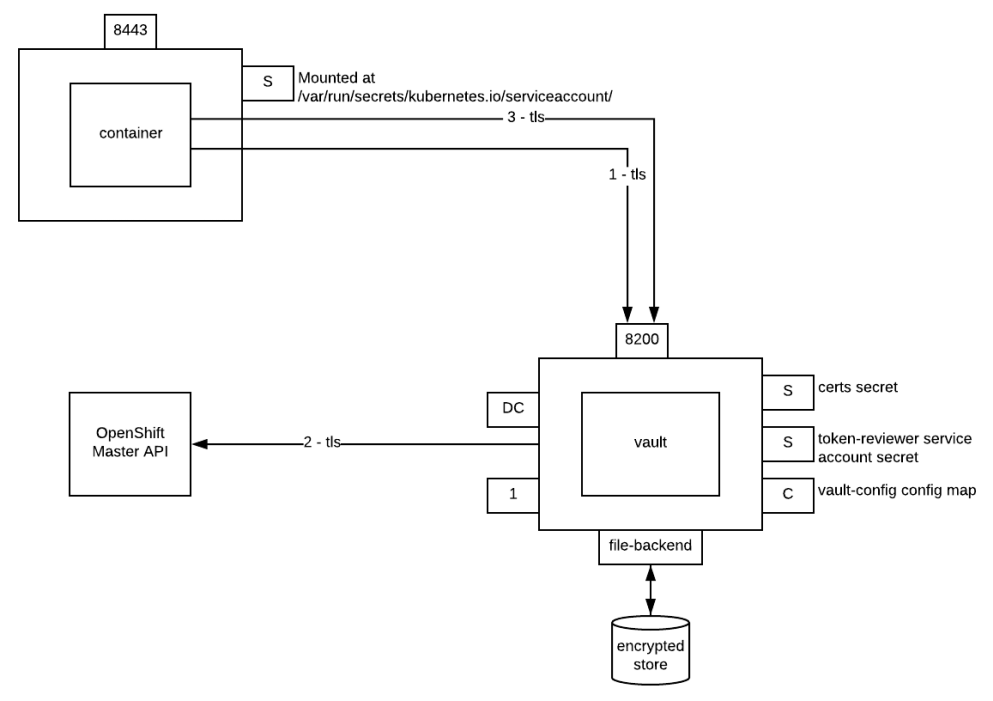
\includegraphics[width=1\linewidth]{kubauth.png}
	\caption[Kubernetes Authentifizierung]{Vault mit Kubernetes Authentifizierung \cite{kubauth}}
	\label{fig:kubauth}
\end{figure}

Neben der LDAP Authentifizierung werden von Vault noch eine Reihe weiterer Authentifizierungsschnittstellen unterstützt. Diese Schnittstellen sind nicht Teil der Evaluierung, werden aber der Vollständigkeit halber hier aufgelistet:\cite{vaultauth}
\begin{itemize}
	\item \textbf{\ac{AWS}:} Der Authentifizierungsdienst des Cloud Anbieters \ac{AWS}
	\item \textbf{Microsoft Azure:} Der Authentifizierungsdienst des Cloud Anbieters Microsoft Azure
	\item \textbf{Google Cloud:} Der Authentifizierungsdienst des Cloud Anbieters Google
	\item \textbf{\acs{JWT}/\acs{OIDC}:} \ac{JWT} in Verbinung mit \ac{OIDC}, einer Authentifizierungsschicht die auf das Protokoll OAuth 2.0 aufsetzt
	\item \textbf{Kubernetes:} Kubernetes verfügt auch über einen eigenen, software-tokenbasierten Authentifizierungsdienst. Die Kopplung von Vault und der Kubernetesdistribution OpenShift ist in Abbildung \vref{fig:kubauth} dargestellt. Weiterführende Informationenen zum genauen Ablauf finden sich in Quelle \cite{kubauth}.
	\item \textbf{GitHub:} Der Authentifizierungsdeinst der Onlineplattform GitHub. GitHub wird dazu verwendet vernetzt und versioniert an Softwarprojekten zu arbeiten.\cite{githubs}
	\item \textbf{\acs{RADIUS}:} \ac{RADIUS} 
	\item \textbf{\acs{TLS} Zertifikate:} X.509 Zertifikate die auch zur Authentifizierung verwendet werden können
	\item \textbf{Token:} Kommen zum Beispiel bei Kerberos zum Einsatz (siehe Kapitel \vref{subsec:token})
	\item \textbf{Benutzername \& Passwort:} In Vault integrierte Benutzerverwaltung
\end{itemize}

Im Abbildung \vref{fig:vaultauth} ist dargestellt wie der Autorisierungsablauf mit Vault funktioniert, wenn die klassische Authentifizierung mit Benutzername und Passwort gewählt wird.

\begin{figure}[h]
	\centering
	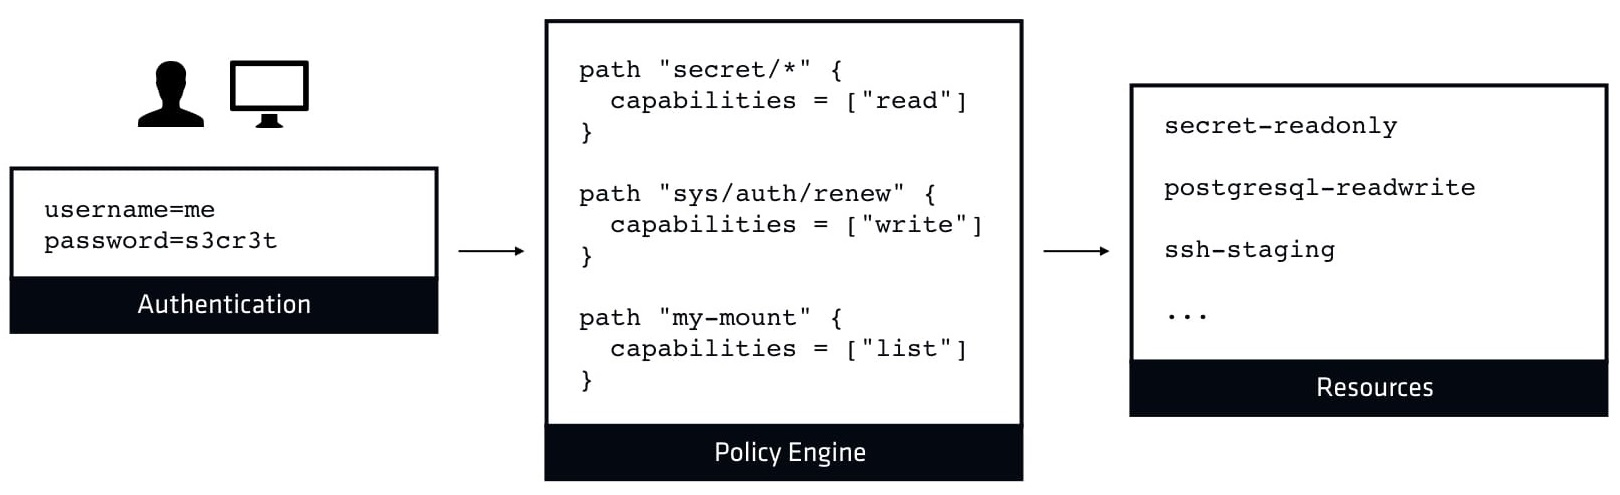
\includegraphics[width=1\linewidth]{vaultauth.jpg}
	\caption[Vault Autorisierung]{Ablauf der Vault Autorisierung \cite{vaultauth2}}
	\label{fig:vaultauth}
\end{figure}

\textbf{Zwischenfazit:} Die Verwendung von LDAP als Authentifizierungsdienst funktioniert wie beschrieben und ermöglicht es somit, Vault in Umgebungen mit existierender Benutzerverwaltung durch LDAP, mit relativ kleinem Konfigurationsaufwand zu integrieren. Weitere Authentifizierungsdienste müssten noch getestet werden.

\subsubsection{\acs{PKI} Integration} 
Zur Evaluierung der \ac{PKI} Integration von Vault wird auf die Authentifizierung mit \ac{TLS} Zertifikaten umgestellt. Dieser Schritt ist nicht nötig, liefert aber einen weiteren Anwendungsfall zum Testen der Funktionalität der Integration. Zuerst wird eine \ac{CA} benötigt welche dann verwendet werden kann um weitere Zertifikate zu beglaubigen. Zu diesem Zweck wird das quelloffene Programm OpenSSL verwendet. Zuerst wird ein Schlüsselpaar nach dem kryptographischen Standard RSA erzeugt\\\inline|sudo openssl genrsa -out rootCA.key 4096|\\ mit dem Kommando\\\inline|openssl req -x509 -new -nodes -key rootCA.key -sha512 -days 1024 -out rootCA.pem|\\ wird dann ein Zertifikat erzeugt, welches dann als \ac{CA} verwendet werden kann. Dieses Zertifikat wird dann auf allen Servern der Infrastruktur zur Liste der vertrauenswürdigen Zertifikaten hinzugefügt. Mit Hilfe dieses Zertifikats können nun Client Zertifikate erstellt werden die dann zur Authentifizierung beim Vault-Server verwendet werden können. Zu diesem Zweck wird wieder ein RSA Schlüsselpaar erzeugt um daraus dann Zertifikate zu erstellen, die von der \ac{CA} beglaubigt werden. Für den Consul-Server sieht es so aus:\cite{openssl}\\\inline|openssl x509 -req -in consul.csr -CA rootCA.pem -CAkey rootCA.key -CAcreateserial -out consul.crt -days 500 -sha512|\newline
Zur Integration in Vault wird eine sogenannte Intermediate\ac{CA} (intermediate ist englisch für Zwischenglied) erstellt. Dieser Schritt wird aus Sicherheitsgründen empfohlen. Nun wird das Zertifikat und der private Schlüssel der Intermediate\ac{CA} zu Vault hinzugefügt und es wird die \ac{PKI} Funktionalität aktiviert. Mit Hilfe dieser Funktionalität lassen sich nun neue Benutzerzertifikate erstellen oder neue \ac{TLS}-Zertifikate zur verschlüsselten Kommunikation und jegliches weitere Anwendungsbeispiel für X.509 Zertifikate. Zum testen dieser Funktionalität kann das Skript in Listing \vref{lst:skript} verwendet werden, bin dem von Vault ein Zertifikat angefordert wird welches eine Gültigkeitsdauer von 10 Minuten hat. Wie in Kapitel \vref{subsec:cloud} beschrieben ist eine solche Funktionalität im bereich Cloud Computing sehr hilfreich im Zusammenhang mit dynamischer Zertifizierung.  


\begin{lstlisting}[caption={[Skript PKI] Shell Skript zum Erstellen eines neuen Serverzertifikats unter Verwendung der Vault \ac{PKI}}, label=lst:skript, captionpos=b, basicstyle=\ttfamily] 
#!/bin/bash

# export location of vault server to environment
export VAULT_ADDR='https://vault.local:8200'

# log into vault unsing certificates
vault login -method=cert -client-cert=/home/user/Dokumente/certs/web.pem -client-key=/home/user/Dokumente/certs/web.key name=web

# generate certificate with 10 minutes validity and save it in /etc/ssl/certs/web-certs.tmp
vault write pki/issue/short-web common_name=web.local > /etc/ssl/certs/web-certs.tmp

# seperate key and certificate from output and save it in two different files
sed -n '/certificate/,/-----END/ p' /etc/ssl/certs/web-certs.tmp | sed 's/[^-]*-/-/' > /etc/ssl/certs/web-cert.crt
sed -n '/private_key/,/-----END/ p' /etc/ssl/certs/web-certs.tmp | sed 's/[^-]*-/-/' > /etc/ssl/certs/web-cert.key

# remove temporary output file
rm -f /etc/ssl/certs/web-certs.tmp

# restart webserver and revoke vault token to end session
vault write auth/token/revoke-self value=true
systemctl restart httpd

\end{lstlisting}

Dieses Skript kann als Cronjob alle fünf bis zehn Minuten ausgeführt werden und lässt damit die lückenlose verschlüsselte Kommunikation mit dem Webserver zu und dies unter Verwendung von sehr kurzlebigen \ac{TLS}-Zertifikaten. 

\textbf{Zwischenfazit:} Die PKI Integration mit Vault funktioniert wie beschrieben. Im verwendeten Anwendungsbeispiel ist die Rückgabe des Zertifikats als reiner Text jedoch relativ unpraktisch, da die Ausgabe noch mit in weiteren Schritten zur Verwendung durch den Web-Server aufbereitet werden muss. Eine Ausgabe in einem Format wie \ac{JSON} oder als einzelne Dateien, ließe eine einfachere Weiterverarbeitung zu.

\subsubsection{Weitere Funktionen}

Einige Funktionen sind sehr einfach zu testen oder ergeben sich schon aus den vorangegangenen Schritten, so zum Beipiel das ver- und entsiegeln von Vault. Nachdem Vault installiert und initialisiert wurde, existieren wie in Kapitel \vref{subsubsec:instv} beschrieben fünf Entsiegelungsschlüssel und ein Root-Token. Um eine installierte Vault Instanz zu starten müssen drei der fünf Entsiegelungsschlüssel zur Verfügung stehen. Die Werte sind konfigurierbar und können auch noch nach der Initialisierung verändert werden. Es ist also möglich einer weiteren vertrauten Person einen Entsiegelungsschlüssel auszustellen und/oder die Mindestanzahl der benötigten Schlüssel herauf oder herab zu setzten. Die Schlüssel werden durch ihre Besitzer eingegeben nachdem sie das Kommando\\\inline| vault operator unseal|\\abgesetzt haben. Die Ausgabe nach Eingabe des ersten Schlüssels wird in Listing \vref{lst:unseal} dargestellt. Jede weitere Eingabe zählt den Index im Feld ``Unseal Progress`` um eins hoch bis der Wert unter dem Feld ``Threshold`` erreicht ist. 
\begin{lstlisting}[caption={[Entsiegelungsprozess] Erster Schritt im Entsiegelungsprozess von Vault}, label=lst:unseal, captionpos=b, basicstyle=\ttfamily] 
Unseal Key (will be hidden): 
Key                Value
---                -----
Seal Type          shamir
Sealed             true
Total Shares       5
Threshold          3
Unseal Progress    1/3
Unseal Nonce       74b3babc-7387-a571-801a-d7ba06667ac3
Version            0.9.5
HA Enabled         true
\end{lstlisting}
Sollte es zu einem Sicherheitsvorfall kommen und die Gefahr bestehen, dass Geheimnisse abgegriffen werden, kann bei rechtzeitigem Erkennen des Vorfalls mit dem Kommando\\\inline|vault operator seal|\\von allen autorisierten Benutzern, Vault für jegliche Interaktion gesperrt werden. Nachdem der Vault-Server-Prozess beendet wurde oder Vault per Kommando versiegelt wurde kann erst wieder zugeriffen werden wenn er wie oben Beschrieben entsiegelt wird. Mit dieser Funktionalität ist ein \textbf{Notfallplan} bei einem Sicherheitsvorfall gegeben.

Die Auditlogfunktion kann durch das Kommando \inline|vault audit enable [file socket syslog]| aktiviert werden. Dabei wird mit den Schlüsselwörtern ``file``, ``socket`` und ``syslog`` das Ziel des Auditlogs angegeben.

Um die Verfügbarkeit von Vault zu erhöhen, kann die \textbf{Hochverfügbarkeitsfunktion} aktiviert werden und der Vault-Server Dienst kann auf mehreren Servern gleichzeitig laufen. Die tatsächliche Schwachstelle im Bezug auf die Verfügbarkeit ergibt sich jedoch auch dem Key-Value Speicher im Hintergrund. Bei der Wahl des Speichers sollte darauf geachtet werden, dass die Technologie über Ausfallsicherheitsoptionen verfügt. Wie in Listing \vref{lst:unseal} zu sehen ist wird der Status der Hochverfügbarkeitsfunktion in der Ausgabe unter dem Feld ``HA Enabled`` gezeigt.\\

\begin{figure}[h]
	\centering
	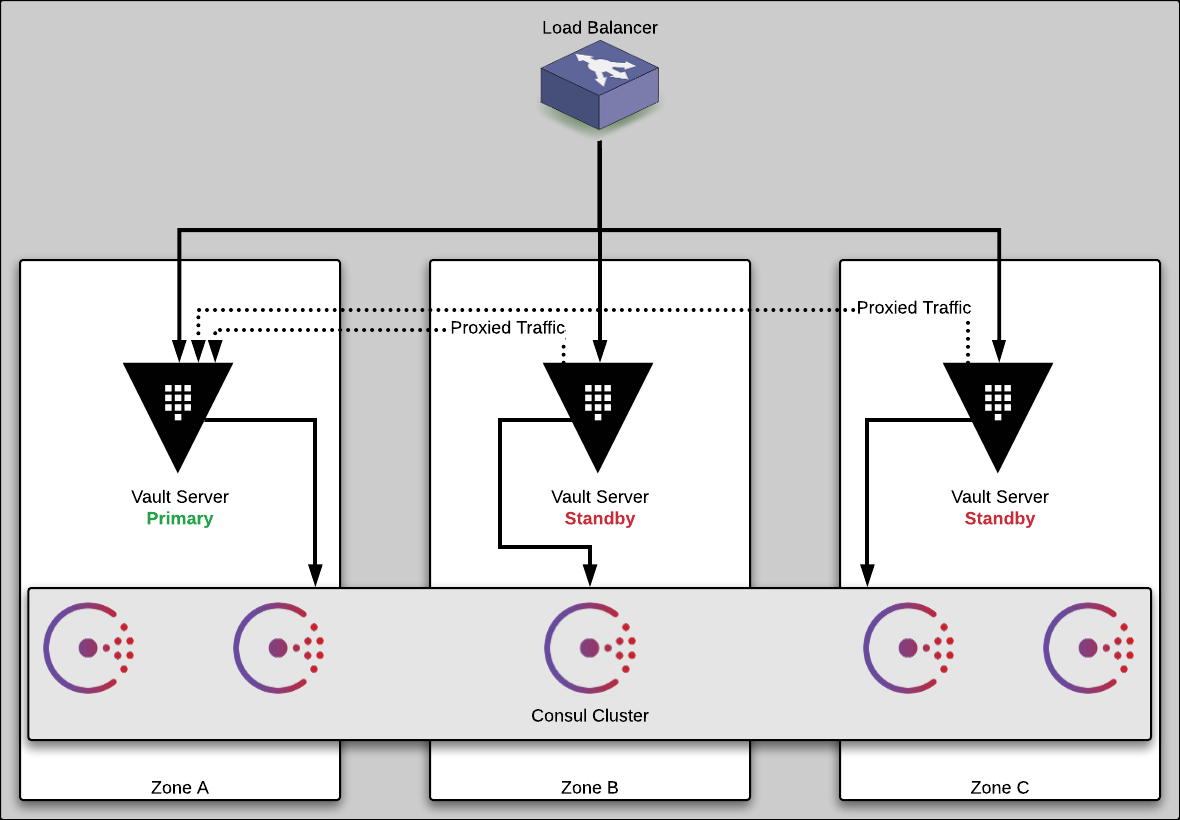
\includegraphics[width=1\linewidth]{vaultha.png}
	\caption[Vault High Availability]{Hochverfügbarkeits-Setup mit drei Vault Servern und einem Consulcluster über mehrere Verfügbarkeitszonen\cite{vaultha}}
	\label{fig:vaultha}
\end{figure}

Ein Beispiel für einen derartigen Anwendungsfall ist in Abbildung \vref{fig:vaultha} dargestellt. Die Darstellung zeigt einen Hochverfügbarkeitsaufbau von Vault mit einem Consulcluster als Storage Backend. Der Load Balancer prüft welcher Vault aktiv ist und vermittelt alle Anfragen an ihn. Sollte beim aktiven Server eine Fehlfunktion auftreten wird automatisch einer der beiden übrigen Server aktiv. Hochverfügbarkeitslösungen über mehrere Standorte sind nur in der kostenpflichtigen Version von Vault verfügbar. 
 
\newpage
\section{Fazit und Ausblick}
\label{sec:ausblick}

Die Anforderungen die Großunternehmen an das Secrets Management ihrer \ac{IT}-Infrastruktur stellen, können durch historisch Gewachsene Umgebungen heute oft nur mit einer Vielzahl an Softwareelementen erreicht werden. Oft ist die Umstellung auf neue Softwareprodukte sehr teuer und die Migration der Zugriffsregeln und Authentifizierungsmethoden ist eine große Hürde. Der Trend zur Verlagerung von Diensten in die Cloud und die Angst der Unternehmen Abgehängt zu werden führt oft dazu, dass an den Sicherheitskonzepten gespart wird. Vault ist ein Produkt, dass einige Probleme die mit dem Umzug in die Cloud aufkommen erfolgreich lösen kann. Die Software kann aber auch in Umgebungen die nicht mit Cloud Diensten arbeiten eine wertvolle Erweiterung sein. Dort wo Funktionen wie Verschlüsselung, sichere Passwortspeicherung und Zertifikatausstellung einer Automatisierung bedürfen, weil sie aktuell durch einen Flickenteppich an kleinen Anwendungen und Skripten realisiert sind, kann Vault einen großen Vorteil bringen.

Vor allem dann, wenn bereits ein funktionierendes Authentifizierungssystem im Einsatz ist, lässt sich Vault relativ problemlos in das bestehende System integrieren und stellt schon allein durch die starke verschlüsselte Ablage von Zugangsdaten einen Vorteil gegenüber herkömmlichen Systemen dar. Auch die Transportverschlüsselung, die bei Vault zum Standardrepertoire gehört kann unter Umständen einen deutlichen Sicherheitsvorteil bieten. 
Die Problematik die sich daraus ergibt, dass eine fortwährende Authentifizierung gegenüber Vault stattfinden muss bleibt jedoch bestehen und lässt sich, nicht abschließend lösen. Der Einstiegspunkt um einen Sitzungstoken von Vault zu erhalten ist weiterhin ein kritischer Punkt und es muss auf die verwendete Authentifizierungssoftware vertraut werden. Die In Kapitel \vref{sec:grund} besprochenen Probleme und Gegenmaßnahmen bleiben also Teil des Secrets Management und können durch Vault lediglich auf tieferen Ebenen verbessert werden.

Für den Produktivbetrieb gibt es unter der Addresse \url{https://www.vaultproject.io/uides/operations/index.html} einige nützliche Anwendungsfälle die bei der Umsetzung sehr hilfreich sein können. Die Dokumentation ist sehr ausführlich und hilfreich bei der Realisierung von verschiedenen Szenarien wie etwa dem Aufbau einer Hochverfügbarkeitslösung von Vault. Sobald zusätzliche Softwarekomponenten notwendig werden (zum Beispiel Storage Engine) werden in den Anwendungsbeispielen allerdings keine Softwareprodukte von Drittanbietern beschrieben. Die Agenda von Hashicorp den eigenen Softwarestack in dieser Beziehung zu bevorzugen ist deutlich erkennbar.

Während der Evaluierung ließ sich das Kommandozeilenwerkzeug mit dem Vault auf Server- und Clientseite angesprochen wird, relativ komfortabel verwenden. Anwender werden sich aber eher schwer tun mit einem Kommandozeilenwerkzeug zu arbeiten. Seit Version 0.10 von Vault ist die graphische Oberfläche von Vault Teil der quelloffenen Version. Die Evaluierung hat zu einem Zeitpunkt stattgefunden, als die Oberfläche nur in der kostenpflichtigen Version zur Verfügung stand und konnte aus diesem Grund nicht bewertet werden. 



%%%%%%%%%%%%%%%%%%%%%%%
%%%%%%%%%%%%%%%%%%%%%%%
%%% end main document
%%%%%%%%%%%%%%%%%%%%%%%
%%%%%%%%%%%%%%%%%%%%%%%
\newpage
\appendix
\Urlmuskip=0mu plus 1mu
\bibliographystyle{plain}
\bibliography{literatur}

\end{onehalfspacing}
\end{document}

%%%%%%%%%%%%%%%%%%%%%%%%%%%%%%%%%%%%%%%%%%%%%%
%%%%%%%%%%%%%%%%%%%%%%%%%%%%%%%%%%%%%%%%%%%%%%
%%%%%%%%%%%%%%%%%%%%%%%%%%%%%%%%%%%%%%%%%%%%%%
%%%%%%%%%%%%%%%%%%%%%%%%%%%%%%%%%%%%%%%%%%%%%%

